\documentclass{scrreprt} % <= Druckversion: "scrbook", Bildschirmversion: "scrreprt"
\newcommand\bcor{12mm} % <= Bindungskorrektur für Druckversion
\usepackage{osm-thesis}


\usepackage{ellipsis} % Leerraumoptimierung
\usepackage{booktabs} % Tabellenstriche unterschiedlicher Stärke
\usepackage{tabularx} % Automatische Zeilenumbrüche
\usepackage{tablefootnote}
\newcommand{\ra}[1]{\renewcommand{\arraystretch}{#1}}
\usepackage{minted} % Farbige Hervorhebung von Quellcode
\RequirePackage{csquotes} % Loaded later because of minted

%%%%%%%%%%%%%%%%%%%%%%%%%%%%%%%%%%%%%%%%%%%%%%%%%%%%%%%%%%%%%%%%%%
\usepackage[edges]{forest} % Verzeichnisbäume

\definecolor{folderbg}{RGB}{124,166,198}
\definecolor{folderborder}{RGB}{110,144,169}
\newlength\Size
\setlength\Size{4pt}

% TODO Use real icons
\tikzset{%
	folder/.pic={%
		\filldraw [draw=folderborder, top color=folderbg!50, bottom color=folderbg] (-1.05*\Size,0.2\Size+5pt) rectangle ++(.75*\Size,-0.2\Size-5pt);
		\filldraw [draw=folderborder, top color=folderbg!50, bottom color=folderbg] (-1.15*\Size,-\Size) rectangle (1.15*\Size,\Size);
	},
	file/.pic={%
		\filldraw [draw=folderborder, top color=folderbg!5, bottom color=folderbg!10] (-\Size,.4*\Size+5pt) coordinate (a) |- (\Size,-1.2*\Size) coordinate (b) -- ++(0,1.6*\Size) coordinate (c) -- ++(-5pt,5pt) coordinate (d) -- cycle (d) |- (c) ;
	},
}
\forestset{%
	declare autowrapped toks={pic me}{},
	pic dir tree/.style={%
		for tree={%
			folder,
			font=\ttfamily,
			grow'=0,
		},
		before typesetting nodes={%
			for tree={%
				edge label+/.option={pic me},
			},
		},
	},
	pic me set/.code n args=2{%
		\forestset{%
			#1/.style={%
				inner xsep=2\Size,
				pic me={pic {#2}},
			}
		}
	},
	pic me set={directory}{folder},
	pic me set={file}{file},
}
%%%%%%%%%%%%%%%%%%%%%%%%%%%%%%%%%%%%%%%%%%%%%%%%%%%%%%%%%%%%%%%%%%

\usepackage[multiple]{footmisc} % Trennung mehrerer Fußnoten durch Kommata
% Requires \usepackage[hyperfootnotes=false,...]{hyperref}, see https://tex.stackexchange.com/a/35060

\usepackage{wrapfig}
\usepackage{subcaption}

%%%%%%%%%%%%%%%%%%%%%%%%%%%%%%%%%%%%%%%%%%%%%%%%%%%%%%%%%%%%%%%%%%
% Import SVG directly via Inkscape-pdf_tex-Export
\usepackage{import}
\graphicspath{{images/}}
\newcommand{\executeiffilenewer}[3]{%
	\ifnum\pdfstrcmp{\pdffilemoddate{#1}}%
	{\pdffilemoddate{#2}}>0%
	{\immediate\write18{#3}}\fi%
} 
\newcommand{\includesvg}[1]{%
	\executeiffilenewer{#1.svg}{#1.pdf}%
	{inkscape -z -D --file=#1.svg %
		--export-pdf=#1.pdf --export-dpi=72 --export-latex}%
	\input{#1.pdf_tex}%
}
%%%%%%%%%%%%%%%%%%%%%%%%%%%%%%%%%%%%%%%%%%%%%%%%%%%%%%%%%%%%%%%%%%

% ABOUT
\newcommand{\hpitype}{Masterarbeit}
\newcommand{\hpiauthor}{Jan-Henrich Mattfeld}

% und Implementierung	
\newcommand{\hpititle}{%
	Entwurf einer %
	einheitlichen Middleware zur %
	Policy-Durchsetzung in %
	Multi-Cloud-Infrastrukturen}
\newcommand{\hpititleother}{Design and Implementation of a Unified Middleware for Policy Enforcement in Multi-Cloud Infrastructures} % <= das Studienreferat verlangt einen deutschen UND englischen Titel

\newcommand{\hpisupervisor}{Max Plauth, Prof.\,Dr.\,Andreas Polze}
\newcommand{\hpichair}{Fachgebiet für Betriebssysteme und Middleware}
\newcommand{\hpiexternalsupervisor}{}
\newcommand{\hpiexternal}{}
\newcommand{\hpidate}{\today}

% DOCUMENT
%\KOMAoption{draft}{true} % <= z.B. zum "Debuggen" der Overfull-Boxes und schnellerem Kompilieren https://tex.stackexchange.com/a/49369
\bibliography{literature/bibliography}

\begin{document}
	\selectlanguage{ngerman}

	% Einband
	\pagenumbering{alph}
	\ifisbook\begin{titlepage}
	\setlength{\evensidemargin}{0.5\evensidemargin+0.5\oddsidemargin}
	\setlength{\oddsidemargin}{\evensidemargin}

	\centering

	\raisebox{-0.5\height}{
\includegraphics[width=5.5cm]{images/hpi_logo_black.pdf}}
	\hspace*{.2\textwidth}
	\raisebox{-0.5\height}{
\includegraphics[width=4cm]{images/uni_logo_black.pdf}}
	
	\vspace*{4\baselineskip}
	{\usekomafont{subject}\hpitype}\par
	
	\vfill
	{\usekomafont{title}\hpititle\par}
	\vspace*{\baselineskip}
	{\usekomafont{subtitle}\hpititleother}\par
	
	\vfill
	{\textbf{\phantom{\iflanguage{ngerman}{von}{by}}} \\
	 \smallskip\usekomafont{author}\hpiauthor}\par
	
	\vfill
	\phantom{\begin{minipage}{\textwidth}
	{\textbf{\iflanguage{ngerman}{Betreuung}{Supervisors}}\\
	\usekomafont{publishers}\smallskip\hpisupervisor\\ \textit{\hpichair}\\ \smallskip\textbf{\normalfont\hpiexternalsupervisor}\\ \textit{\hpiexternal}}
	\end{minipage}}
	
	\vfill
	{\usekomafont{date}\iflanguage{ngerman}{Hasso-Plattner-Institut an der Universität Potsdam}{Hasso Plattner Institute at University of Potsdam}}\par
	\vspace*{\baselineskip}
	{\usekomafont{date}\hpidate}\par
	
\end{titlepage}\fi
	\ifisbook\cleardoubleemptypage\fi

	% (Haupt-)Titelseite, Abstract, ggf. Danksagung & Inhaltsverzeichnis
	\pagenumbering{roman}
	\begin{titlepage}
	\centering

	\raisebox{-0.5\height}{
\includegraphics[width=5.5cm]{images/hpi_logo_srgb.pdf}}
	\hspace*{.2\textwidth}
	\raisebox{-0.5\height}{
\includegraphics[width=4cm]{images/uni_logo_srgb.pdf}}

	\vspace*{4\baselineskip}
	{\usekomafont{subject}\hpitype}\par
	
	\vfill
	{\usekomafont{title}\hpititle\par}
	\vspace*{\baselineskip}
	{\usekomafont{subtitle}\hpititleother}\par
	
	\vfill
	{\textbf{\iflanguage{ngerman}{von}{by}}\\ 
		\smallskip\usekomafont{author}\hpiauthor}\par
	
	\vfill
	{\textbf{\iflanguage{ngerman}{Betreuung}{Supervisors}}\\ 
		\usekomafont{publishers}\smallskip\hpisupervisor\\ \textit{\hpichair}\\ \smallskip\textbf{\normalfont\hpiexternalsupervisor}\\ \textit{\hpiexternal}}
	
	\vfill
	{\usekomafont{date}\iflanguage{ngerman}{Hasso-Plattner-Institut an der Universität Potsdam}{Hasso Plattner Institute at University of Potsdam}}\par
	\vspace*{\baselineskip}
	{\usekomafont{date}\hpidate}\par

	\setcounter{page}{1}

\end{titlepage}


	\ifisbook\cleardoubleemptypage\fi
	% \null\vfil
\begin{otherlanguage}{ngerman}
\begin{center}\textsf{\textbf{\abstractname}}\end{center}

Cloud-Ressourcen spielen eine entscheidende Rolle in den aktuellen und zukünftigen IT-Strategien von Unternehmen aller Größen. Gleichzeitig entstehen zentrale Herausforderungen in Hinblick auf Vertraulichkeit und Zuverlässigkeit, sowie Portabilität der eigenen Daten und Anwendungen. Mit dem Inkrafttreten der Datenschutz-Grundverordnung und immer neuen Datenlecks ist das Thema hochaktuell.

Durch die intelligente Kombination von Private- und Public-Cloud-Infrastruktur treten wir diesen Herausforderungen entgegen. Wir geben einen Überblick über aktuelle kommerzielle und akademische Multi-Cloud-Projekte. Dabei identifizieren wir fehlende SLA- und Cloud-Schnittstellen-Standards als größte Risiken.

Als Lösungsvorschlag entwickeln wir einen Multi-Cloud-Anwendungs-Broker auf den Ebenen IaaS und CaaS. Dabei dient das TOSCA-Simple-Schema zur Anwendungs- und SLA-Spezi\-fi\-ka\-tion. Wir diskutieren den Aufwand der Cloud-Teststellungen und den Einsatz der Multi-Cloud-Bibliothek Apache Libcloud. Die Leistungsfähigkeit der Lösung demonstrieren wir anschließend in einem Testaufbau mit OpenStack, AWS, Docker und Hyrise-R.

Wir versetzen Cloud-Kunden in die Lage, ihre Anforderungen anbieter- und technikunabhängig zu formulieren und durchzusetzen. Unsere Lösung automatisiert die Einhaltung von Datenschutz-, Qualitäts- und Kostenzielen. Damit ist das Projekt einzigartig und ergänzt die bisherigen Beiträge im SSICLOPS-Kontext.

\end{otherlanguage}
\vfil\null




	\tableofcontents
	\cleardoublepage

	% Textteil
	\pagenumbering{arabic}
	\chapter{Einleitung}

% New Mesosphere Data Center Operation System (DC/OS)
%
% Kubernetes as a Service, No SLAs, but transparent Deployment to several clouds
%
%Seamless Edge and Multi-Cloud Operations — Unifying multiple cloud providers and private datacenters has been the holy grail for infrastructure and operations teams since the birth of cloud computing. Gartner estimates 9 in 10 enterprises will adopt Hybrid Infrastructure Management within two years. Enterprises want the flexibility to choose where to run their applications based on cost, speed to market, and security & compliance considerations. Distributing today’s applications and a growing set of data services across multiple infrastructures (including private and edge computing environments) helps guarantee quality of service and uptime. Bursting workloads to the cloud, disaster recovery across locations, and simplified management of edge compute and remote offices is now effortless with DC/OS as your unified control plane. DC/OS 1.11 allows you to pool public cloud, private datacenter, and edge compute resources into a single logical computer and intelligently schedule workloads anywhere from a unified user interface.
%
% https://mesosphere.com/blog/dcos-1_11-overview/

Cloud-Angebote sind allgegenwärtig und werden mittlerweile von einer Mehrzahl deutscher Unternehmen genutzt. Laut \emph{Statista} setzten bis 2016 mindestens fünfundsechzig Prozent aller Betriebe entsprechende Lösungen ein \cite{bitkom:2017:cloud-nutzung-unternehmen};
%https://de.statista.com/statistik/daten/studie/177484/umfrage/einsatz-von-cloud-computing-in-deutschen-unternehmen-2011/
besonders gefragt sind Infrastrukturdienste, wie Rechenleistung und Speicher. Gleich darauf folgen Softwareangebote und E-Mail-Hosting. Etwas abgeschlagen bleiben Plattformdienste wie Datenbanken und Ausführungsumgebungen \cite{destatis:2016:cloud-nutzung-unternehmen-einsatzzweck}. %https://de.statista.com/statistik/daten/studie/381830/umfrage/einsatzzwecke-von-cloud-computing-in-unternehmen-in-deutschland/
Der Trend zur Cloud wird sich vermutlich fortsetzen: So vervierfacht sich das prognostizierte Marktvolumen mit Cloud-Services bis 2020 auf über sechzehn Milliarden Euro allein im deutschen B2B-Markt \cite{isg:2017:cloud-ausgaben-2020}. %
%https://de.statista.com/statistik/daten/studie/165458/umfrage/prognostiziertes-marktvolumen-fuer-cloud-computing-in-deutschland/

Cloud-Angebote sind für Unternehmen aller Größen attraktiv: Die Anschaffung eigener Infrastruktur entfällt, genauso wie deren Wartung durch eigenes Personal. Stattdessen lassen sich Ressourcen und Anwendungen einfach per Selfservice buchen und sind anschließend über das Internet von überall erreichbar. Der Umfang gebuchter Leistungen lässt sich meist frei skalieren. Da die Angebote oft in kleinem Takt und verbrauchsgenau abgerechnet werden, ergeben sich so theoretisch Vorteile bei Flexibilität und Kosteneffizienz.

Demgegenüber stehen Vorbehalte bezüglich Datenschutz, denn die gemietete Infrastruktur teilen sich mehrere Kunden. Durch Sicherheitslücken wie \emph{Spectre} und \emph{Meltdown} werden eigentlich geschützte Speicherbereiche angreifbar \cite{Kocher2018spectre, Lipp2018meltdown}. Nach aktuellem Stand existierten diese Lücken mehr als ein halbes Jahr in fast jedem x86-System, und damit in fast jeder Cloud \cite{techcrunch:2018:spectre-meltdown-tier-2-cloud-vendors}. Eine sichere Mandantentrennung war also nicht mehr gewährleistet \cite{aws:2018:security-bulletin}. 
%https://aws.amazon.com/security/security-bulletins/AWS-2018-013/
Aber auch durch Unachtsamkeit werden Cloud-Datenspeicher immer wieder der Öffentlichkeit zugänglich \cite{upguard:2017:breach-alteryx, upguard:2017:breach-centcom, kromtech:2018:breach-fedex}.
%Amazon S3 Datenlecks

Zugleich fordert aktuelle Gesetzgebung wie die Datenschutz-Grundverordnung unter anderem die Verarbeitung von personenbezogenen Daten europäischer Kunden ausschließlich innerhalb der EU \cite{eu:2016:bdsvg}. %http://data.consilium.europa.eu/doc/document/ST-12399-2016-INIT/en/pdf %Anbieter sind in der Pflicht. Haftung auch Gegenüber Endkunden, mit denen eigentlich keine direkte Geschäftsbeziehung besteht. Löschpflicht. Wo sind die Daten physisch? Portabilität Cloud->Kund und Cloud->Cloud
%Weitere Anforderungen Diese Regelungen sind keineswegs auf Europa begrenzt. Gleiches in der USA (Amazon Gov CLoud)
Gut neunzig Prozent aller Unternehmen achteten folglich bei der Auswahl eines Cloud-Providers auf Rechts- und Server-Standorte in Deutschland \cite{gartner:2017:cloud-market}. 

Auch vorhandene Softwarelizenzen können den Umzug verhindern. Zum Beispiel Oracle oder Microsoft-OEM-Lizenzen verbieten die Übertragung in eine Cloud-Umgebung \cite{microsoft:2017:licensing, oracle:2018:licensing}. So müssen möglicherweise Teile der Infrastruktur lokal vorgehalten werden.

Für gut fünfzig Prozent der interessierten Unternehmen außerdem unabdingbar: individuelle Dienstgütevereinbarungen, sogenannte \emph{Service Level Agreements (SLAs)} \cite{bitkom:2017:cloud-nutzung-unternehmen-auswahlkriterien}.
%https://de.statista.com/statistik/daten/studie/545924/umfrage/kriterien-bei-der-auswahl-eines-cloud-providers-in-deutschen-unternehmen/
Dies lässt jedoch einige der weltweit größten Cloud-Anbieter außen vor -- Amazon und Microsoft teilen sich seit 2016 über fünfzig Prozent des weltweiten Umsatzes mit Infrastrukturdiensten \cite{gartner:2017:cloud-market}. Die Vertragsbedingungen beider Anbieter sind jedoch nicht verhandelbar. %https://de.statista.com/statistik/daten/studie/754647/umfrage/marktanteile-am-umsatz-mit-infrastructure-as-a-service-weltweit/

Laut Gartner wollen daher 70 Prozent aller Unternehmen bis 2019 eine Multi-Cloud-Strategie umsetzen \cite{gartner:2017:cloud-market-multicloud-trend}. Zusätzlich zu einer privaten Cloud werden hierbei auch Dienste aus weiteren öffentlichen Angeboten genutzt. Vorteil ist eine höhere Flexibilität, um für jede Anforderung die ideale Cloud wählen zu können. Kriterien sind zum Beispiel die Einhaltung gesetzlicher Anforderungen, spezielle SLAs, höhere Ausfallsicherheit und die Preisgestaltung der Anbieter. Multi-Cloud birgt aber auch einige Herausforderungen:

% XKCD on Meltdown and Spectre: https://xkcd.com/1938/

% Capgemini WHitepaper "from boring to sexy" Multi Cloud ist Trend."
%
%https://www.computerwoche.de/a/migration-in-die-cloud-so-vermeiden-sie-fehler,3327477
%
%https://www.computerwoche.de/a/der-trend-geht-zur-multi-cloud,3332352
%
%https://www.computerwoche.de/a/mit-der-multi-cloud-zur-digitalen-infrastruktur,3331691
%
%https://www.computerwoche.de/a/was-ist-multi-cloud-der-naechste-schritt-im-cloud-computing,3331658
%
%https://www.gartner.com/doc/reprints?id=1-4KKGOTA&ct=171115&st=sb%3fsrc=so_5703fb3d92c20&cid=70134000001M5td

\begin{itemize}
	\item Portabilität eigener Anwendungen
	\item Cloud-Provider-spezifisches Know-how
	\item Höherer IT-Verwaltungsaufwand der Ressourcen
	\item Managementaufwand, wie der Vergleich von Compliance-Richtlinien
	\item Keine oder geringere preisliche Skaleneffekte
	\item Überwachung der heterogenen Cloud-Landschaft
	\item Durchsetzung der eigenen Sicherheits- und Datenschutzrichtlinien
\end{itemize}

\noindent
Um diese Herausforderungen automatisiert abzumildern, eignet sich eine \emph{Cloud-Management-Plattform (CMP)} mit integriertem Anwendungs-Broker. Deren Marktsituation ist allerdings unübersichtlich und in großer Bewegung. Bereits im letzten Jahr wurden einige vielversprechende Lösungen von Cloud-Infrastruktur-Providern aufgekauft \cite{gartner:2017:cloud-market-multicloud-trend}. Die CMPs sind nun selbst Software-as-a-Service-Angebote und proprietär. Die eigentlichen Vorteile Flexibilität und Unabhängigkeit werden so ad absurdum geführt.

Unabhängige Lösungen sind mehrheitlich ausgelaufene akademische Forschungsprojekte. Auf den aktuellen Cloud-Markt und technische Neuerungen wie Container sind diese nicht mehr anwendbar. Aufgrund der vorherigen Forschungsergebnisse ergibt sich jedoch folgende Hypothese:

%CMPs ändern sich ständig. selbst während dieser arbeit sind Anbieter ausgeschieden, aufgekauft oder grundlegend verändert. cost als neues feature. kein echtes brokering, sondern self-service und monitoring.

\begin{verse}
	{Eine unabhängige, auf offenen Standards basierende CMP kann die Vorteile der Cloud mit aktuellem Datenschutz vereinen.}
\end{verse}

\noindent 
Das EU-geförderte Forschungsprojekt \emph{Scalable and Secure Infrastructures for Cloud Operations (SSICLOPS)} identifiziert Private- und Hybrid-Cloud-Umgebungen als zukünftigen Treiber des ITK-Markts \cite{ssiclops:2015:d6.1-project-presentation}. Im Rahmen dieses Projektes entwickeln wir einen Multi-Cloud-Broker. Alle Ergebnisse basieren auf Open-Source-Technologien und sollen, wenn möglich, an die Ursprungsprojekte zurückfließen. Der Broker soll Organisationen und Unternehmen als Cloud-Nutzer emanzipieren und besonders den kommerziellen Wert der Lösung herausstellen.

%https://ssiclops.eu/wp-content/uploads/SSICLOPS_D6.1_final.pdf
%Private and hybrid cloud technology is a key enabler  for  future  ICT  growth

Da SLAs und weitere Rahmenbedingungen oft nicht verhandelbar sind, muss die Optimierung der Cloud-Nutzung in Eigenregie erfolgen.  Die vorgestellte CMP erlaubt die Nutzung bestimmter Anbieter, obwohl SLAs  nicht eingehalten werden: zum Beispiel lässt sich eine höhere Ausfallsicherheit durch Kombination mehrerer Anbieter erreichen. Nebenbei entsteht so ein Notfallplan zum Weiterbetrieb bei Ausfall oder Kündigung eines Cloud-Providers.

Das folgende Kapitel klassifiziert Cloud-Angebote anhand bestimmter Eigenschaften und Service-Ebenen. Außerdem geben wir eine Einführung in datenschutzrechtliche Fragen und Risiken in Zusammenhang mit Cloud-Bereit\-stel\-lungs\-model\-len.

Anschließend entwickeln wir passende Policys und entsprechende Schemata. Diese sollen von dem eigens entwickelten Multi-Cloud-Broker verwendet werden. Er verteilt auch ältere -- nicht Cloud-native -- Anwendungen über verschiedene Cloud-Provider auf IaaS- und CaaS-Ebenen und optimiert die Cloud-Landschaft anschließend fortlaufend. Dabei beachtet er SLAs und Datenschutzanforderungen. Für diesen Vorschlag bewerten wir akademische und kommerzielle Projekte mit ähnlicher Zielsetzung.

Der Implementierungsteil vergleicht verschiedene Multi-Cloud-Bibliotheken. Auf Basis von Apache \emph{libcloud} entwickeln wir eine CMP, die das Multi-Cloud-Brokering übernimmt. Auch Implementierungshürden und Besonderheiten der verschiedenen Clouds werden beschrieben. Als Beispielanwendung dient dabei die verteilte Forschungsdatenbank \emph{Hyrise-R}. Auch die Entstehung eines \emph{OpenStack}-Testbeds als Beispiel einer Private-Cloud wird besprochen. Es folgt eine abschließende Bewertung des Konzepts.

% Bei Benkanntwerden von Spectre/Meltdown waren noch keine Fixes, wohl aber POCs verfügbar. Eigene Anwendungen hätten also sofort von der öffentlichen in eine private Cloud umgezogen werden müssen, oder -- falls das auf grund mangelnder Portabilität nicht möglich ist -- abgeschaltet. Notfallplan?

%- Klassifizierung von Cloud-Angebote und Risiken
%- Datenschutzrechtliche Bewertung von Daten 
%- Portabilität von Anwendungen für einfache Cloud-übergreifende Migrationen
%- Entwicklung von entsprechenden Policys und einem Schema
%- Vorschlag eines eigens entwickelten Multi-Cloud-Brokers, der auch nicht cloud-native Anwendungen über verschiedene Cloud-Provider auf IaaS, CaaS und PaaS-Ebenen in Hybriden Umgebungen verteilt und managt. Dabei beachtet er SLAs und Datenschutzanforderungen.
%- Related work: Gegenüberstellung Verschiedener kommerzieller und akademischer Projekte mit ähnlicher Zielsetzung. Fehlende Eigenschaften
%Wie nützlich ist Apache libcloud (oder generell eine Multi-Cloud Library? Vergleich!)
%- Einbindung bisher nicht cloud-nativer Anwendungen am Beispiel von hyrise-R
%- Technische Betrachtung des Prototypen mit Hyrise-R und OpenStack als Grundlage im Rahmen von SSCICLOPS
%- Future Work und Bewertung des Prototypen
%
%Nur Teile einer CMP umgesetzt. Identity spielt hier z.\,B. keine Rolle. 
	\chapter{Hintergrund -- Chancen und Herausforderungen in der Cloud}

Dieses Kapitel definiert die grundlegenden Charakteristika eines Cloud-Dienstes, die verschiedenen Service-Ebenen, Liefermodelle, Akteure und ihre Verantwortlichkeiten. Aus diesen Definitionen entwickeln sich zwei grundlegende Herausforderungen der Cloud-Nutzung:

\begin{enumerate}
	\item Datenschutz/Vertraulichkeit
	\item Portabilität von Daten und Anwendungen
\end{enumerate}

Je nach Cloud-Nutzung ergeben sich hierfür verschiedene Lösungsansätze, die im weiteren Verlauf gegeneinander abgegrenzt werden.


\section{Eigenschaften eines Cloud-Dienstes}

Unabhängig von Liefer- und Servicemodell zeichnet sich ein Cloud-Dienst durch bestimmte Merkmale aus. Konkret definieren übereinstimmend \emph{NIST Cloud Computing Reference Architecture}, \emph{IETF} und \emph{BSI-Grundschutzkatalog} \cite{nist:2011:reference-architecture, ietf:2015:reference-framework, bsi:2014:grundschutz} folgende Eigenschaften:

\begin{description}
	
	\item[On-demand Self-Service] Ressourcen werden vom Cloud-Kunden selbstständig über ein Portal oder eine Webschnittstelle angefordert und anschließend automatisch provisioniert.
	
	\item[Breitbandzugriff] Die gemieteten Ressourcen werden über ein Netzwerk, typischerweise das Internet, bereitgestellt. Der Zugriff erfolgt über Standardschnittstellen wie HTTP; kann also von überall erfolgen und ist im Regelfall nicht auf bestimmte Geräte oder Software beschränkt.
	
	\item[Geteilte Infrastruktur] Die zugrunde liegenden physischen Ressourcen werden virtualisiert und flexibel unter mehreren Kunden aufgeteilt. Die vorhandene Hardware wird so möglichst optimal ausgelastet. Gleichzeitig ergeben sich hierdurch Datenschutzbedenken; die Daten einzelner Mandaten müssen streng getrennt sein.
	
	\item[Elastizität] Durch einen hohen Grad an Automatisierung werden Ressourcen zeitnah zur Verfügung gestellt. Lastspitzen können ohne manuelle Eingriffe abgefangen werden.
	
	\item[Messbarkeit] Die Ressourcennutzung ist messbar und wird kontinuierlich überwacht. Abgerechnet wird zum Beispiel nach CPU-Zeit, Speicherkapazität oder Anzahl genutzter IP-Adressen.
	
\end{description}

Von klassischem IT-Outsourcing grenzt es sich durch Self-Service, Skalierbarkeit und geteilte Infrastruktur ab. Diese Eigenschaften bieten Kunden theoretisch Flexibilität und Kostenvorteile. In der Lösungssuche sollen diese positiven Aspekte möglichst erhalten bleiben.


\section{Service-Ebenen}

Je nach Auswahl des Cloud-Angebots lassen sich verschiedene Kernebenen unterscheiden. Diese bauen jeweils aufeinander auf und verbergen die Komplexität der darunterliegenden Ebenen. Je weiter sich die Abstraktion von der physischen Ebene entfernt, desto weniger lässt sich das Angebot durch den Kunden anpassen:

\begin{description}
	
	\item[Infrastructure as a Service (IaaS)] Die klassische Bereitstellung von Infrastruktur wie virtuellen Maschinen, Speicherplatz und Netzwerkdienstleistungen. Der Kunde ist hier selbst für die Administration zuständig, muss also Einrichtung und Wartung von Betriebssystemen, Treibern und Middleware selbst verantworten.
	
	\item[Container as a Service (CaaS)] Variante von IaaS, bei dem eine Laufzeitumgebung für Container bereitgestellt wird. In diesen sind alle Abhängigkeiten der Gastanwendung vorinstalliert und laufen auf dem bereits initialisierten Kernel des Hosts. Vorteil ist eine höhere Elastizität durch geringeren Overhead. Im Folgenden ist bei der Erwähnung von IaaS immer auch CaaS inkludiert.
	
	\item[Platform as a Service (PaaS)] Hier übernimmt der Cloud-Provider die Bereitstellung der zuvor genannten Bestandteile. Der Kunde betreibt auf dieser Ebene eine selbst erstellte Anwendungssoftware. Über Bibliotheken und Schnittstellen des Cloud-Providers greift er auf Laufzeitumgebungen, Datenbanken und Entwicklungswerkzeuge zu.
	
	\item[Function as a Service (FaaS)] Auch als \emph{Serverless-Computing} populär: Entgegen dem Namen arbeiten auch hier noch Server, diese sind für den Kunden jedoch weitestgehend unsichtbar. Es stellt eine Evolution des PaaS-Modells dar und ist besser als FaaS beschrieben -- der Kunde lädt nur noch Quellcode in die Cloud. Dieser wird nun Ereignis-getrieben ausgeführt, skaliert und abgerechnet. Im Gegensatz zu vielen PaaS-Angeboten fallen im Ruhebetrieb keine weiteren Kosten an \cite{crisp:2016:serverless-infrastructure}.
	
	\item[Software as a Service (SaaS)] Eine bestehende Anwendungssoftware wird komplett vom Cloud Provider bezogen. Die Verantwortlichkeit des Kunden beschränkt sich meist auf kleinere Anpassungen, Nutzerverwaltung und das Einspielen eigener Daten.
	
\end{description}

Besonders interessant für eigene Entwicklungen im Rahmen des \emph{SSICLOPS}-For\-sch\-ungs\-kon\-tex\-tes sind dabei die Ebenen IaaS und CaaS \cite{ssiclops:2015:d6.1-project-presentation}. Sie bieten genug Flexibilität, um die Fragestellung mit folgenden Produkten zu erproben:

\begin{enumerate}
	\item \emph{OpenStack} als zentraler Infrastrukturprovider
	\item Die verteilte Forschungsdatenbank \emph{Hyrise-R} als Beispielanwendung
\end{enumerate}

Cloud-Provider bieten darüber hinaus weitere Hilfs- und Verwaltungsdienste. Diese betreffen vor allem Konfiguration, Provisionierung, Monitoring und Abrechnung. Hierzu zählen aber auch Sicherheit, Vertraulichkeit und Portabilität. Diese drei Querschnittsthemen sollen im Zusammenhang mit den Dienstebenen weiter untersucht werden.

Die \emph{NIST}-Klassifizierung unterscheidet hier speziell weitere, teils externe, Akteure wie Cloud-Auditoren und -Carrier \cite{nist:2011:reference-architecture}. Dieser Einteilung folgt die Arbeit nicht. Stattdessen konzentriert sie sich auf die direkte Beziehung zwischen Cloud-Kunden und -Provider. Beide haben Risiken und Verantwortlichkeiten, die im nächsten Abschnitt besprochen werden.


\section{Risiken}

Moderne IT-Infrastruktur ist hochkomplex. Allein hierdurch ergibt sich ein großes Potenzial für Bedrohungen. Im Cloud-Computing steigt das Risiko durch gemietete und geteilte Infrastruktur weiter \cite{csa:2016:cloud-top-threats, Pearson:2010:issues-arising-cloud, 2011:takabi:security-challenges}. Zusätzlich zu allgemeinen Risiken sollen mögliche Auswirkungen auf folgende Eigenschaften beschrieben werden:

\begin{enumerate}
	\item Verfügbarkeit
	\item Vertraulichkeit
	\item Integrität
	\item Portabilität
\end{enumerate}

Abhängig vom Einsatzzweck des geplanten Cloud-Services resultieren die Fragen: Welche Informationen und Prozesse müssen geschützt werden, welche Bedrohungen sind zu erwarten? Damit ist nicht nur Sicherheit gemeint, sondern alle Risiken, die den Erfolg eines Cloud-Projektes oder einer Organisation darüber hinaus bedrohen. Möglicher Schaden muss im Voraus berechnet werden. Zu verarbeitende Daten sollten kategorisiert werden; dem \emph{BSI} folgend sind diese vier Abstufungen denkbar \cite{bsi:2014:Anforderungskatalog}:

\begin{enumerate}
	\item Privat- , Geschäfts- und Dienstgeheimnisse gemäß \emph{§§\,203} und \emph{353\,b StGB}
	\item Personenbezogene Daten gemäß \emph{§\,3 Absatz\,1 BDSG}
	\item Verschlusssachen
	\item Sonstige Daten (weder Kategorie 1, noch 2, noch 3)	
\end{enumerate}

Verschlusssachen der Kategorie drei meint hier alle Daten, deren Verlust, Veränderung oder unrechtmäßige Herausgabe sich nachteilig auswirken könnte. Die Abgrenzung der letzten beiden Kategorien erscheint oft schwierig, muss jedoch für jeden betriebenen Cloud-Service abgewogen werden.

Diese Arbeit konzentriert sich auf die Risiken, die direkt von Cloud-Kunden und \mbox{-Providern} auf den Ebenen IaaS und PaaS beeinflusst werden können. So ist zum Beispiel die Sicherheit der Client-Geräte, von denen auf die Cloud-Dienste zugegriffen wird entscheidend, aber nicht Teil dieser Betrachtung.

Aus der Datenkategorie ergeben sich Anforderungen an die Risikoanalyse. Je höher und je wahrscheinlicher ein potenzieller Schaden, desto aufwendiger und teurer sollte die Absicherung ausfallen. Grundsätzlich lassen sich zwei Kategorien von Risikofaktoren unterscheiden \cite{monjur:2017:security-taxonomy}:

\begin{itemize}
	\item Menschlich
	\item Technisch
\end{itemize}

Menschliche Fehlhandlungen sind entweder absichtlich oder unabsichtlich. Dies können Fehlinterpretation von SLAs, Manipulationen, Angriffe durch \emph{Social-Engineering} oder schlicht Inkompetenz sein. Im Cloud-Computing treten diese Risiken verstärkt auf, da die Infrastruktur von Dritten betreut wird. Auch Gesetzesänderungen zählen zu diesen Risiken. Viele lassen sich durch passende Standardprozesse, Notfallpläne, Rechtemanagement und Audits vermindern.

Technisch gilt Ähnliches: Klassische Risiken, wie der Ausfall von Hardware, wird vom Cloud-Provider vor dem Kunden verborgen. Speziell auf Cloud-Projekte bezogen eröffnen sich aber auch neue Angriffsflächen wie die Cloud-Plattform selbst. Die Virtualisierungsebene kann durch mangelhafte Mandantentrennung Datenlecks öffnen. Viele Cloud-Provider arbeiten mit proprietären Protokollen, die Portabilität ist also eingeschränkt. Umso herausfordernder wird ein Notfallplan, der den Ausfall des Anbieters abfangen soll.

All diese Risiken müssen durch SLAs und Policys abgebildet werden. Diese sollten maschinenlesbar sein, um automatisiert angewandt und überprüft zu werden. Detaillierte Leitfäden hierzu bieten BSI und CSA \cite{bsi:2014:Sicherheitsrichtlinie, csa:2015:star}. Insgesamt hängt das Risiko stark vom Bereitstellungsmodell ab, also von Standort und Nutzerkreis der Infrastruktur.


\section{Bereitstellungsmodelle und Multi-Cloud-Architekturen}

Cloud-Angebote können von öffentlichen Anbietern oder intern bereitgestellt werden. Weiter differenzieren lassen sich die Angebote nach Nutzerkreis, mit dem die Infrastruktur geteilt wird und Anzahl der genutzten Clouds \cite{petcu:2014:cloud-taxonomy, grozev:2014:cloud-taxonomy}:

\begin{description}
	
	\item[Public Cloud] Alle Leistungen werden von einem öffentlichen Anbieter bezogen. Dies sind zum Beispiel Amazon, Microsoft und Google. Die Infrastruktur wird unter mehreren Kunden flexibel aufgeteilt.
	
	\item[Private Cloud] Eine eigen- oder fremd-betriebene Infrastruktur mit exklusivem Zugriff für einen Kunden. Wird die Private Cloud im eigenen Datencenter betrieben, erhalten Kunden größtmögliche Vertraulichkeit. Gleichzeitig müssen aber Überkapazitäten vorgehalten werden, wodurch der Kostenvorteil kleiner als bei Nutzung öffentlicher Angebote ausfallen kann.
	
	\item[Hybrid Cloud] Heterogene Infrastruktur mit Bestandteilen in privaten und öffentlichen Cloud-Umgebungen. Die öffentliche Cloud übernimmt hier oft die Speicherung großer Datenmengen und das Abfangen von Lastspitzen.
	
	\item[Community-Cloud] Ein Zusammenschluss von Unternehmen, Behörden oder For\-sch\-ungs\-ein\-rich\-tun\-gen, die gemeinsam eine Cloud-Infrastruktur betreiben. Die beteiligten Cloud-Anbieter bilden eine freiwillige \emph{Föderation} der gemeinsamen Ressourcen.
	
	\item[Multi-Cloud] Eine Erweiterung der Hybrid Cloud: Die Leistungen werden nicht nur aus einer privaten und einer öffentlichen Cloud bezogen, sondern explizit aus mehreren. Wichtiger Unterschied zur Föderation: Die Multi-Cloud-Umgebung wird vom Cloud-Anwender initiiert und verwaltet. Beteiligte Cloud-Provider wirken nicht aktiv mit und sind sich ihrer Partizipation meist nicht einmal bewusst.
	
\end{description}

Von allen beschriebenen Bereitstellungsmodellen ist die Multi-Cloud am flexibelsten. Je nach technischen und nicht-funktionalen Anforderungen können Bestandteile der Cloud-Anwendungen in einer möglichst passenden Umgebung ausgeführt werden. Der Aufwand ist in diesem Modell allerdings auch am höchsten, denn der Auswahlprozess für einen Cloud-Provider muss für alle Anbieter einzeln durchlaufen werden.

Hierbei werden die Rahmenbedingungen geprüft; unter anderem Kosten, Standort der Rechenzentren und anwendbare Gesetzesgrundlage. Hinzu kommen technische Herausforderungen, da die Portabilität von Daten und Anwendungen zwischen verschiedenen Cloud-Providern oft eingeschränkt ist.

Um eine automatisierte Bewertung der Cloud-Angebote vorzunehmen, müssen die Anforderungen möglichst genau spezifiziert werden. Dazu dienen Policys und SLAs. Der folgende Abschnitt zeigt die wichtigsten Beispiele und erläutert ihre Bedeutung im Kontext der Arbeit.


\section{Policys, SLAs und Optimierungsgrößen}

Cloud-Nutzer und -Provider haben gegenseitige Erwartungen, die abgestimmt werden müssen. Innerhalb von Unternehmen gelten außerdem bestimmte Regeln zum Umgang mit Informationen (\emph{Compliance}), angelehnt an die Gesetzeslage und externe Zertifizierungen wie ISO 27001 \cite{iso:2013:27001}. Über die gesetzlichen Regelungen hinaus kann ein Unternehmen weitere Ziele setzen: Kosteneinsparungen oder der Einsatz klimafreundlicher Energie.

Dieser Abschnitt definiert die verschiedenen Formen für den späteren Einsatz im Multi-Cloud-Broker. Er liefert Verweise zu Standards und entwickelt Beispiele für den späteren Prototyp. Wir unterscheiden für die Verwendung im Broker:

\newpage

\begin{description}
	\item[Policys] Maßnahmenorientiert, Regeln, \\
	z.\,B. \emph{Datenverarbeitung ausschließlich innerhalb der EU}
	\item[Service Level Agreements] Ergebnisorientiert, Vereinbarungen zur Dienstgüte, \\
	z.\,B. \emph{Verfügbarkeit über ein Jahr $99,99\,$\%}
	\item[Optimierungsgrößen] Gewichtete sonstige Ziele der Cloud-Nutzung, \\
	z.\,B. \emph{minimale Gesamtkosten bei Berücksichtigung aller Policys und SLAs}
\end{description}

Alle drei Themen beeinflussen sich gegenseitig: Richtlinien werden -- wenn möglich -- in das SLA übernommen, alle übrigen setzt der Cloud-Kunde selbst um. Eine Überschneidung ist ebenfalls möglich: Neben einer \emph{99,99\,\%-Uptime}-Klausel kann es zusätzlich eine Replikations-Policy geben; beide bestimmen die Verfügbarkeit.

Typischerweise enthalten die Policys und SLAs weitere Informationen zu Vertragspartnern, Eskalationsmanagement, Vertragsstrafen und Laufzeit. Da diese Punkte für die Untersuchung nicht relevant sind, konzentrieren wir uns auf die in SLAs enthaltenen Metriken, sogenannte \emph{Service-Level-Objectives (SLOs)}. Wir nehmen zusätzlich einen vereinfachten Gültigkeitszeitraum über den gesamten Lebenszyklus eines Services an.

Hierarchien innerhalb der Policys bleiben ebenso außen vor: So könnte es zum Beispiel die strategische Entscheidung geben, Daten nur innerhalb bestimmter Länder zu verarbeiten -- gleichzeitig gilt auf dem Service-Level eine weitere Einschränkung auf die EU. Wir konzentrieren uns direkt auf letzteren Fall. Weitere Ziele wie die Ausfallsicherheit unterscheiden sich ebenso individuell pro Service.

Sowohl Policys als auch SLAs sollten bestimmte Eigenschaften erfüllen. Eine Erweiterung der \emph{SMART-Kriterien} \cite{doran:1981:smart-goals} für Cloud-Computing könnte wie folgt aussehen:

\begin{enumerate}
	\item Erfüllbar
	\item Verständlich
	\item Nützlich
	\item Angemessen\,/\,Allgemein akzeptierbar
	\item Reproduzierbar
	\item Messbar
	\item Beeinflussbar
	\item Finanziell tragbar
\end{enumerate}

Einige Metriken sind typisch für Dienstleistungsverträge, zum Beispiel der Durchsatz. Andere wie die Löschfrist sind durch neuere Gesetzesvorgaben entstanden oder betreffen wie die Nachhaltigkeit das Image eines Unternehmens. Alle lassen sich grob in Kategorien sortieren; Allgemein, Performance, Zuverlässigkeit, Datenmanagement, Sicherheit, Datenschutz.

Die folgende Auflistung zeigt die wichtigsten Policys und SLA-Metriken. Sie erläutert außerdem die Bedeutung für diese Arbeit:

\begin{description}
	
	\item[Redundanz] Wie oft soll ein bestimmter Dienst repliziert und parallel betrieben werden? Dieser Wert beeinflusst maßgeblich die Verfügbarkeit.	
	
	\item[Geo-Lokation] Geografischer Standort des Datencenters. Mögliche Einschränkungen aufgrund von Datenschutzgesetzen. Beeinflusst außerdem die Antwortzeiten des Services.
	
	\item[Elastezität] Wie schnell können neue Ressourcen bereitgestellt oder wieder heruntergefahren werden? In einer IaaS-Umgebung ist dies meist der Zeitraum vom Start einer neuen VM bis zur Einsatzbereitschaft. Unsere servicebezogene SLA misst zusätzlich die Zeit, bis eine neue Instanz tatsächlich Teil des Clusters ist, und einen Teil der Last abnimmt.
	
	\item[Agilität] Effizienzmetrik: Wie feingranular können die Ressourcen skaliert werden? Die Bedeutung für den Cloud-Broker ist vernachlässigbar: Die verschiedenen Ressourcen-Angebote der Cloud Provider müssen im Voraus normalisiert werden. Zur Laufzeit werden sie nur noch verglichen.
	
	\item[Durchsatz] Wie viele Anfragen können (pro Sekunde) bearbeitet und beantwortet werden? Die Anfrage ist vorher zu definieren. Typischerweise wird nicht das Mittel aller Anfragen gemessen, sondern von 99\% -- Ausreißer sind erlaubt.
	
	\item[Latenz] Zeit um eine Anfrage zu beantworten. Beeinflusst von Geolokation, Datenbankstandort und Auslastung.
	
	\item[Datenstandort] Datenbank und Anwendung sollten immer in unmittelbarer Nähe zueinander platziert werden. Dies wirkt sich positiv auf die Latenz einer Anfrage aus, kann aber zu höheren Kosten führen.
	
	\item[Bevorzugen eigener Ressourcen] Solange in der eigenen Private-Cloud Ressourcen vorhanden sind, sollten diese zuerst -- vor öffentlichen Drittangeboten -- genutzt werden. Auch hier müssen zusätzlich Leistungsmetriken wie die Latenz berücksichtigt werden.
	
	\item[Verfügbarkeitszeit (Uptime)] Zeitanteil, innerhalb dessen Anfragen den übrigen Metriken entsprechend beantwortet werden. Üblicherweise ab 99,9\,\% eines Jahres. Könnte durch die gemeinsame Nutzung mehrerer Clouds erhöht werden.
	
	\item[Wiederherstellungszeit] Durchschnittlicher Zeitraum, nachdem ein Service nach Ausfall wieder vollständig zur Verfügung steht. Dies beinhaltet die zügige und korrekte Beantwortung aller Anfragen sowie die Erfüllung aller übrigen SLOs.
	
	\item[Backup] Eine Sicherung von IaaS-Instanzen oder Datenbankinhalten in bestimmten Abständen verteilt auf mehrere Speicherorte. In diesem Fall bezogen auf einen Service. Außerdem zu beachten: die benötigte Zeit zur Wiederherstellung.
	
	\item[Zugriffskontrolle] Lesende und schreibende Aktionen auf Ressourcen müssen durch ein Identitäts- und Zugriffsmanagement geregelt und protokolliert werden. Dies ist jedoch ein eigenes Thema, das hier nicht weiter behandelt wird. Außerhalb der Administrationsebene implementiert die ausgeführte Anwendungssoftware oft eigene Mechanismen.
	
	\item[Benachrichtigungssystem] Ein Trigger-Action-System: Bei Eintreten bestimmter Ereignisse wie dem Ausfall einer Systemkomponente soll automatisiert eine festgelegte Nachricht versendet werden, dies können eine E-Mail oder ein REST-Call sein.
	
	\item[Speichertypen] unterscheiden sich deutlich in Zugriffszeit, Transferrate, verfügbarer Kapazität, Zuverlässigkeit und Preis. IaaS-Angebote lassen oft die Wahl zwischen SSD und HDD. Auf PaaS-Ebene kann auch die Art des Datenbankservices gemeint sein: In-Memory, hybrid oder klassisch.
	
	\item[Löschfrist] Handels- und Steuerrecht verlangen für einige Daten die rechtssichere Speicherung und Revisionssicherheit. Umgekehrt gilt für personenbezogene Daten laut BDSG auch eine Löschpflicht, sobald die Daten nicht mehr für den ursprünglichen Zweck benötigt werden. Dies kann meist nur auf Datensatzebene durchgesetzt werden.
	
	Eine befristete Bereitstellung von Service-Instanzen ist jedoch auch denkbar. Die Löschung könnte dann im Rahmen von \emph{Aufräum}-Zyklen erfolgen und Kosten durch Überprovisionierung sparen.
	
	\item[Verschlüsselung] Je nach Service-Ebene entweder die Festplatte einer IaaS-Instanz oder der PaaS-Datenbankservice. Eine Verschlüsselung der Übertragungswege wird angenommen. Auf Datensatz- und Anwendungsebene sind eigene Implementierungen, unabhängig von der CMP, üblich.
	
	\item[Kosten] Verbunden mit einem SLA bieten Cloud-Provider Ressourcen zu einem bestimmten Preis. Dieser ist oft dynamisch, daher sollte eine Optimierung nach Prüfung aller anderen \emph{harten} Kriterien erfolgen.
	
	Den beteiligten Abteilungen hilft die Anzeige der Kosten pro Service. Die CMP sollte Auslastung und Preise dienstübergreifend optimieren.
	
	\item[Nachhaltigkeit/Energiequelle] Nutzt das Datencenter Ökostrom, wenn ja in welchem Umfang? Auch denkbar: Ausgleichsleistungen des Anbieters.
	
\end{description}

Diese Ziele gelten immer zusätzlich zu allgemeinen Hardware- und Softwareanforderungen. Voraussetzung für die Durchsetzung sind weitreichende Zusatzinformationen zum gegenwärtigen Zustand der Cloud und Umgebungsinformationen wie aktuellen Preisen. Innerhalb des \emph{Policy-Enforcement-Points}, also zum Beispiel der CMP, müssen diese Zusatzinformationen gesammelt werden.

Herausforderung hierbei: Die wichtigsten Cloud-Provider veröffentlichen die nötigen Informationen zu ihrem Angebot meist weder maschinenlesbar, noch in einem einheitlichen Format. Policys und besonders SLAs sind typischerweise in natürlicher Sprache verfasst. Für den Einsatz in einem Broker sollten sie jedoch streng formalisiert und damit maschinenlesbar sein, um automatisiert angewandt und überprüft zu werden.

Das folgende \autoref{cha:broker} zeigt daher -- neben bisherigen Broker-Forschungsarbeiten -- bestehende Schemata zur Darstellung von SLAs. Die weitere Besprechung der Policy-Gestaltung erfolgt im Implementierungsteil in \autoref{cha:implementierung}.

	\chapter{Multi-Cloud-Anwendungs-Broker}
\label{cha:broker}

% Vorteile
% Neue Märkte in anderen Regionen der Welt
% Schnelles Ausrollen neuer Apps
% DevOps geeignet
% Risikoreduzierung
% Reduzierung von (gleichzeitig) Investitionsausgaben und Betriebskosten
% Bestehende Cloud-Deployments mit verwalten-

Um eine Anwendung automatisiert auf verschiedene Clouds zu verteilen, ist ein Broker-Mechanismus nötig. Dieser sollte nach verschiedenen, festzulegenden Kriterien vorgehen. Konkret erfüllt ein Broker in der Regel folgende Aufgaben \cite{gartner:2017:cloud-market-multicloud-trend}:

\begin{enumerate}
	\item Bereitstellen der Ressourcen für eine Applikation; starten einer virtuellen Maschine oder Reservierung von Speicherplatz
	\item Starten der Anwendung auf den vorher reservierten Ressourcen
	\item Verteilen eingehender Anfragen auf gestartete Anwendungs-Instanzen
	\item Management der Ressourcen
\end{enumerate}

\noindent
Zusätzlich sollte der Multi-Cloud-Broker Policys und SLAs auswerten und umsetzen können. Denkbar ist das automatische Re-provisionieren anhand von 

\begin{enumerate}
	\item Lastspitzen oder Ausfällen von Hardware und Netzwerkressourcen 
	%	(Monitoring)
	\item Geänderten Umfeldparametern wie der Gesetzgebung, Preisen oder AGBs
	\item Nutzeränderungen
	\item Vorherigen Broker-Aktionen
\end{enumerate}

\noindent
In einer Community-Cloud könnten Cloud-Provider selbst einen Mechanismus zum Brokering oder zumindest offene APIs bereitstellen. Der Broker wäre also Teil der Cloud. Möglich sind entweder ein zentraler Broker, der direkt auf Cloud-Interna zugreift, oder aber ein Peer-to-Peer-Verbund.\todo{Grafik Architekturübersicht}

Für Multi-Clouds kommen diese Lösungen nicht infrage: Sie bestehen aus mehreren unabhängigen, meist privaten, Cloud-Providern. Aufgrund gegenläufiger Geschäftsinteressen sind diese nicht an einer Föderation mit anderen Anbietern interessiert. Sie werden also weder Interna ihrer Cloud-Plattform anpassen, noch einheitliche APIs bereitstellen.

Stattdessen muss der Broker in einer Multi-Cloud-Umgebung extern bereitgestellt werden. In diesem Fall kann er, entweder als eigenständiger Service in Form einer \emph{Cloud-Management-Plattform} angelegt sein, oder von der verteilten Anwendung selbst implementiert werden. Selbst entwickelte CMPs oder integrierte Broker setzen oft auf Multi-Cloud-Bibliotheken wie \emph{Apache libcloud}. \autoref{sec:bibliotheken} bietet hierzu eine Übersicht aktueller Open-Source-Projekte. 

Folgende weitere Aspekte sollen bei der Betrachtung der CMPs berücksichtigt werden:

\begin{description}
	
	\item[Zielgruppe] 	\emph{Entwickler und Administratoren}: Im Rahmen von DevOps stellen sie verschiedene Ausführungsumgebungen für Entwicklung, Test und Produktion bereit. Dabei nutzen sie die Self-Service-Funktionen der CMPs.
	
						\emph{Management}: Die Auslastungs- und Kostenübersicht ermöglicht weitere Planung. SLAs und Policys werden überwacht und durchgesetzt.
	
	\item[Anwendungen] Grundsätzlich alle interaktiven Anwendungen und Dienste, sowie Stapelverarbeitungsjobs. Diese können verteilt sein. Die CMP muss in diesem Fall z.\,B. die Nähe des Datenspeichers zur Recheneinheit beachten.
	
	Ausgenommen: spezielle Big-Data-Analytics- und Forschungsszenarien, die unter Umständen besondere Features, Rechte und Architekturen benötigen.
	
	\item[Funktionsumfang] Über die grundlegende Provisionierung hinaus sollte die CMP auch bei weiteren Orchestrationsaufgaben unterstützen: (1) Konfiguration, (2) Monitoring und (3) Skalierung \cite{weerasiri:2017:orchestration}.
%	https://dzone.com/articles/cloud-management-roundup-orchestration-vs-paas-vs-cmp
	
	Die Unterstützung aktueller Container-Technologien und Cloud-native-Architekturen ist wünschenswert. Keine Rolle spielt \emph{Bare Metal}: Eine installierte Virtualisierungsschicht oder Container-Laufzeitumgebung wird vorausgesetzt. Die noch jungen \emph{Unikernels} erfordern größere Anpassungen beim Betrieb eigener Anwendungen. Sie sind vielversprechend, aber -- auch aufgrund ihrer noch geringen Verbreitung -- potenzielles Thema weiterer Forschungsarbeiten \cite{plauth:2017:unikernels}.
	
	Die Auswertung der SLAs und Policys ist auf die verteilten Anwendungen selbst beschränkt. Darüber liegende (CMP-Nutzer) oder tiefer gehende Schichten (Service-Nutzer und -Daten) werden extern verwaltet. Damit unterscheidet sich der Ansatz von anderen \emph{SSICLOPS}-Arbeiten, die eine Annotation auf Datenebene mit anschließender Policy-Durchsetzung auf allen Cloud-Schichten vorsehen \cite{ssiclops:d21:secure-data-storage, ssiclops:d22:intercloud-policies}.
		
\end{description}

\noindent
Der folgende Abschnitt gibt eine Übersicht kommerzieller Cloud Management Plattformen sowie bisheriger Forschung zu Inter- und Multi-Cloud-Brokern mit besonderem Blick auf SLAs und Policys. Die vorgestellten Lösungen unterscheiden sich in Architektur, Flexibilität und Funktionsumfang. Die vier anfangs vorgestellten Broker-Basiseigenschaften werden nicht von allen Arbeiten in vollem Umfang erfüllt.

Weiterhin zeigen wir einheitliche Ansätze zu maschinenlesbaren Policy- und SLA-Definitionen. Anschließend entwickeln wir ein Service-Schema für den Multi-Cloud-Einsatz. Es folgen der Vorschlag für ein Broker-Design und passende Matching-Algorithmen.


%%%%%%%%%%%%%%%%%%%%%%%%%%%%%%%%%%%%%%%%%%%%%%%%%%%%
\section{Maschinenlesbare SLA- und Policy-Schemata}%
%%%%%%%%%%%%%%%%%%%%%%%%%%%%%%%%%%%%%%%%%%%%%%%%%%%%

%Service Level Agreement Mediation, Negotiation and Evaluation for Cloud Services in Intercloud Environments vorgelegt von M.Sc. Dipl.-Ing. (FH) Alexander Stanik
Bisherige Arbeiten und Spezifikationen zu Cloud-SLAs beschreiben oft einen (externen) Mediator zwischen Provider und Kunden \cite{stanik:2016:sla-mediation}. Der Fokus liegt dort auf der dynamischen Verhandlung und rechtssicheren Dokumentation von SLAs. Die vorgestellten Schemata sind teils ausgereifte Verhandlungsframeworks \cite{casola:2016:per-service-sla-negotiation}. In diesem Abschnitt untersuchen wir die Verwendbarkeit der bisherigen Arbeiten für den Multi-Cloud-Broker, also vor allem für die Gestaltung der SLOs auf Service-Ebene ohne den erweiterten Kontext wie Unterzeichner und Gültigkeitszeitraum oder Sicherheit.

Außerdem wollen und können wir SLAs nicht verhandeln -- Public-Cloud-Provider bieten Kleinkunden keine individuellen Angebote. Stattdessen sucht der Broker anhand bestimmter Anforderungen eine passende Kombination aus einem oder mehreren Cloud-Angeboten. Die hierzu nötigen Informationen sind nicht in einem einheitlichen Format verfügbar. Die allgemeine Zuverlässigkeit und entsprechende Schadensersatzansprüche sind jedoch an zentraler Stelle\footnote{\url{https://azure.microsoft.com/de-de/support/legal/sla/cloud-services/v1_0/}}\footnote{\url{https://aws.amazon.com/de/ec2/sla/}} öffentlich zugänglich, Preise und Geostandorte sind per API\footnote{\url{https://libcloud.readthedocs.io/en/latest/compute/pricing.html}} abrufbar. In hybriden Umgebungen müssen die Parameter der privaten Cloud selbst ermittelt werden. 

Offen ist der Durchsetzungspunkt der Policys. Soll dies bereits in der CMP oder innerhalb von Plattformdiensten und Anwendungsprogrammen geschehen? Für Benutzer-Policys könnte beides der Fall sein: Die versendeten Anwendungsdaten enthalten Metainformationen zur erlaubten Verwendung. Schon die erste Kontaktstelle der Cloud, zum Beispiel ein Load-Balancer, wertet diese Informationen aus und entscheidet entsprechend für ein Routing, das den Nutzeranforderungen entspricht \cite{henze:2013:requirements-aware}. 
% Towards Data Handling Requirements-aware Cloud Computing

In der Anwendung selbst können diese Metainformationen auch genutzt werden, zum Beispiel zur gewünschten Verschlüsselung oder einer Frist zur automatischen Löschung. Ein besonders auf Performance fokussierter Ansatz ist CPPL \cite{henze:2016:cppl}. Bei System-Policys ist die Performance der Decodierung jedoch nicht entscheidend: Sie findet nur bei Änderungen durch Administratoren statt, nicht bei jedem Datenpaket, das die Cloud erreicht. Folgende Prozessschritte innerhalb des Brokers nutzen die SLA-Schemata \cite{koch:1996:policy-definition}:
%Operational Level (Management, Computational)
%Policy- und Event Definition Language
%Anforderungen->Graph
% [2] T. Koch, C. Krell, and B. Krämer, "Policy definition language for automated management of distributed systems"

\begin{enumerate}
	\item Einlesen der Provider-Angebote
	\item Definieren der Anforderungen auf Anwendungs-Ebene
	\item Abgleichen der Angebote und Installation
	\item Überwachen der Vereinbarungen
	\item Reagieren: Ressourcen umverteilen
	\item Durchsetzen: Schadensersatz einfordern
\end{enumerate}

\noindent
Besonders das Monitoring eines Services ist entscheidend um Ansprüche gegenüber Cloud-Providern durchzusetzen. Letztendlich nutzen aber alle Bestandteile des Brokers SLA-Dokumente. Diese sollten also leicht verständlich und integrierbar sein. Inwieweit sich bisherige Standards für Multi-Cloud-Einsätze eigenen, beschreibt die nächste Auflistung.

\begin{description}
	\item[Web Services Agreement Specification (WS-Agreement)] wurde 2007 unter anderem von IBM als Mitglied des \emph{Open Grid Forums (OGF)} vorgestellt \cite{ogf:2011:ws-agreement}. Das XML-Schema beschreibt SLAs für Web-Services auf \emph{SOAP}-Basis. WS-Agreement ist dabei nur ein Teil der \emph{WS-*}-Spezifikationen -- das Aushandeln der SLAs erfolgt über die Erweiterung \emph{WS-Agreement Negotiation} \cite{ogf:2011:ws-negotiation}.
	
	Im Vergleich ist WS-Agreement oberflächlicher als \emph{WSLA} und fokussiert sich auf den SLA-Lebenszyklus: Es besitzt keine Sprachelemente zur Beschreibung von Metriken, wie logische Operatoren oder Prädikate. Der Sprachumfang ist begrenzt und muss über Erweiterungen ergänzt werden, Listing \ref{listing:ws-agreement} zeigt hierzu ein Beispiel.
	
	Für jeden Praxiseinsatz muss eine domänenspezifische Erweiterung mit entsprechenden Metriken entwickelt werden. Der Einstieg ist insgesamt jedoch leichter als bei \emph{WSLA}. Die Referenzimplementierung ist \emph{WSAG4J}\footnote{\url{http://wsag4j.sourceforge.net}}. Zusätzlich zu \emph{SOAP} existiert auch eine modernere REST-Schnittstelle \cite{feigenbutz:2014:wsag-rest-performance}.

	\begin{listing}[ht]
		\inputminted[firstline=16, lastline=34]{xml}{./src/WS-Agreement.sample.xml}
		\caption{Auszug aus einem erweiterten WS-Agreement; ohne Metainformationen, dem sogenannten \emph{Context}. Das Beispiel zeigt eine Vereinbarung zur Verfügbarkeit eines Webservices. Die \emph{ServiceDescriptionTerms} sind hier noch unvollständig, sie werden mit Laufzeitinformationen wie der IP-Adresse gefüllt. Alle messbaren Eigenschaften eines Services sind unter \emph{ServiceProperties} definiert. \emph{metric1} ist hierbei ein externer Verweis. Die eigentlichen SLOs nehmen Bezug auf die vorher definierten Metriken. Optional sind \emph{Business-Values}, die konkrete Strafzahlungen und Zielerreichungsboni definieren.}
		\label{listing:ws-agreement}
	\end{listing}	
	%https://github.com/Fiware/ops.Sla-framework/blob/master/sla-core/docs/ws-agreement.md Complete Example
	
	\item[Web Service Level Agreement (WSLA)] wurde 2003 von IBM vorgestellt und basiert ebenso wie \emph{WS-Agreement} auf XML \cite{ludwig:2003:wsla, keller:2003:wsla}. Der Fokus liegt hier allerdings stärker auf den Metriken: \emph{WSLA} erlaubt Metrik-Komposita und eingebettete Funktionen. Selbst ohne Erweiterungen lassen sich komplexe Anforderungen über logische Ausdrücke, Prädikate und Makros abbilden.
	
	SLOs unterstützen weitere Angaben zu Mess-Abständen und -Zeiträumen. Möglich sind auch Referenzen auf \emph{WSDL} zur Modellierung von Services selbst. Das Framework ist für beide Vertragspartner gleichermaßen geeignet: \emph{WSLA} modelliert Angebot genauso wie Anforderungen. Überwachung und Auswertung können ausdrücklich auch von einer dritten Partei implementiert werden.

	\item[Topology and Orchestration Specification for Cloud Applications (TOSCA)] dient nicht primär zur Abbildung von SLAs, sondern zur providerunabhängigen Modellierung von Cloud-Services \cite{oasis:2013:tosca}. Ursprünglich ebenfalls als XML-Schema entwickelt, existiert seit 2014 eine vereinfachte Variante auf YAML-Basis \cite{oasis:2018:tosca-simple}. Der Sprachumfang ist viel geringer als bei \emph{WS-Agreement} oder \emph{WSAL}, dafür enthält \emph{TOSCA} einsatzbereite Policy-Basistypen. Listing \ref{listing:tosca-policy} zeigt den Aufbau einer Redundanz-Regel über mehrere Regionen. Die weitere Besprechung erfolgt im nächsten Abschnitt zu Infrastruktur- und Service-Definitionen.
		
	\begin{listing}[ht]
		\inputminted[]{yaml}{./src/TOSCA.policy.sample.yaml}
		\caption{Definition einer TOSCA-Policy im YAML-Format: Der Broker soll mindestens drei Instanzen in den ausgewählten Regionen bereitstellen. Erkennbar sind auch die Vererbung innerhalb der Policy-Typen und bereits vorgegebene Basistypen der TOSCA-Policy-Spezifikation.}
		\label{listing:tosca-policy}
	\end{listing}
	
	%	https://wiki.opnfv.org/display/domino/Policy+in+Tosca
	%https://cloudify.co/2014/07/22/TOSCA-KPIs-monitoring-cloud-management.html

	\item[SLA*] ist im Rahmen von \emph{SLA@SOI} entstanden \cite{kearney:2010:sla-star}. Die Sprache ist ein Beispiel für spezielle Eigenentwicklungen: Eine abstrakte Syntax soll \emph{SLA*} universell und domänenübergreifend einsetzbar machen. Als Besonderheit ist sie dabei unabhängig von einer Auszeichnungssprache. Für diese Arbeit ist sie nicht interessant: Alle Anwendungsfälle sind ein Web-Service oder verwandt, daher eigenen sich die anderen Sprachen ohne Einschränkungen.

\end{description}

\noindent
Sowohl \emph{WS-Agreement} als auch \emph{WSLA} nutzen XML. Sie sind streng formalisiert und durch die verfügbaren Schemata leicht maschinell zu verarbeiten. Außerdem existieren direkte Abbildungen auf \emph{ITIL} und dessen Vertragsobjekte \cite{koehler:2006:itil}. Für Menschen sind beide Ansätze jedoch nur schwer les- und editierbar.
%	Köhler, Peter T.: ITIL: Das IT-Servicemanagement Framework. 2007

\emph{TOSCA} hingegen ist leichter einsetzbar: Durch YAML-Importe lassen sich sprachunabhängig Referenzen abbilden. Daher erübrigt sich auch vorerst die Frage, ob Policy- und Service-Definitionen getrennt erstellt werden müssen. \emph{TOSCA} ermöglicht beides \cite{borgi:2014:tosca-intro}.

%%%%%%%%%%%%%%%%%%%%%%%%%%%%%%%%%%%%%%%%%%%%%%%%%%%%%%%%%%%%%%%
\section{Einheitliche Infrastruktur- und Service-Definitionen}%
%%%%%%%%%%%%%%%%%%%%%%%%%%%%%%%%%%%%%%%%%%%%%%%%%%%%%%%%%%%%%%%

Durch die Definition von SLAs und Policys steht nun fest, wo und wie ein Service bereitgestellt werden soll. Die konkrete technische Umsetzung ist bisher allerdings offen. Oberstes Ziel der Multi-Cloud-Service-Definition ist Portabilität: Die gleiche Anwendung muss auf verschieden Hypervisoren, IaaS/CaaS- und Plattform-Angeboten ausgeführt werden können. Nur so ergeben sich die Vorteile des Multi-Cloud-Ansatzes.

Aber wann eignet sich eine Anwendung für die Nutzung in der Cloud? Je nach Entstehungsgeschichte können sich Softwarearchitektur und Migrationsmaßnahmen grundlegend unterscheiden:

\begin{description}
	
	\item[Klassisch] (Legacy-)Anwendung mit monolithischem Design
	
	\emph{$\Rightarrow$ Ausführungsumgebung portabel bereitstellen, z.\,B. als (Container-)Image}
	
	\item[Web-App] Mehrere, skalierbare Anwendungsteile
	
	\emph{$\Rightarrow$ Zusätzlich die Nutzbarkeit von PaaS-Komponenten prüfen}
	
	\item[Cloud-native] Abhängigkeiten zu proprietären Cloud-Services (interner Broker)
	
	\emph{$\Rightarrow$ Refactoring und Öffnung der App-Schnittstellen zur CMP}
	
\end{description}

\noindent
Gerade bei klassischen, monolithischen Anwendungen ergeben sich architekturbedingt nicht alle Vorteile der Cloud-Nutzung; eine erhöhte Portabilität ist gegeben --  Skalierbarkeit allerdings nicht. Die Entscheidung für Anpassung, Migration oder unveränderten Weiterbetrieb muss also je nach technischer Eignung und langfristiger Bedeutung für das Kerngeschäft abgewogen werden.

Ist die Entscheidung für eine Multi-Cloud-Migration gefallen, muss eine portable Infrastruktur geschaffen werden. Dieser Prozess besteht aus drei wesentlichen Schritten:

\begin{enumerate}
	
	\item Interpretation einer einheitlichen Service-Definition
	\\\emph{(Auswahl von Cloud-Ressourcen und passender Ausführungsform)}
	
	\item Bereitstellen von Infrastruktur-Ressourcen 
	\\\emph{(Virtuelle Maschine, Containerlaufzeitumgebung, Netzwerkspeicher etc.)}
	
	\item Übertragen der Anwendung in die Ausführungsumgebung
	\\\emph{(und initiale Konfiguration sowie Prüfung)}
	
\end{enumerate}

\noindent
SLAs und Policys werden hier noch nicht betrachtet. Der spätere Broker berücksichtigt sie vor allem während der Ressourcenauswahl in Schritt eins. Herausforderungen ergeben sich durch die Heterogenität von Cloud-Schnittstellen und Infrastruktur.

Durch die Marktdominanz von Amazon \emph{AWS} wurden zwischenzeitlich einige der proprietären Formate von Open-Source-Projekten übernommen: zum Beispiel \emph{Amazon Machine Images} (AMI, Cloud-optimierte Images\footnote{\url{https://docs.aws.amazon.com/de_de/AWSEC2/latest/UserGuide/AMIs.html}}) und \emph{CloudFormation} (Infrastruktur- und Service-Definitionen\footnote{\url{https://aws.amazon.com/de/cloudformation/}}). Zielführend ist das jedoch nicht: Die Formate können sich jederzeit ändern, sind speziell auf Amazon-Angebote ausgerichtet und unterstützen im Gegenzug keine Eigenheiten anderer Infrastruktur. Dementsprechend haben sie sich nicht durchgesetzt:

\begin{description}
	
	\item[Ausführungsumgebungen] Innerhalb der Service-Ebenen stehen je nach Cloud-Provider unterschiedliche Ausführungsumgebungen zur Verfügung. Die zugehörige initiale Konfiguration einer neuen Instanz kann über interne Werkzeuge erfolgen oder Drittanbieter einbinden.
	
	Auf Hypervisor- und IaaS-Ebene sind \emph{Cloud Images} wie die von Ubuntu\footnote{\url{https://cloud-images.ubuntu.com/}} inoffizieller Standard. Im Gegensatz zu den Standardausgaben sind sie speziell für den Einsatz in virtuellen Umgebungen vorbereitet. Sie integrieren \emph{Canonicals cloud-init\footnote{\url{https://cloudinit.readthedocs.io/}}}: Die initiale Konfiguration kann hierüber Provider-unabhängig per Konfigurationsdatei und/oder Skript übergeben werden. Optional bindet \emph{cloud-init} über Plugins die Metadatendienste des Providers ein.
	
	Eine ähnliche Verbreitung auf CaaS-Ebene haben \emph{Docker}-Container\footnote{\url{https://www.docker.com/what-docker}}. Besonderheiten sind die zentrale Container-Verwaltung, eine Vielzahl vorgefertigter Basis-Images und Konfigurationsmöglichkeiten per \emph{Dockerfile} und/oder Startparameter\footnote{\url{https://docs.docker.com/engine/reference/builder/}}. Die Container sind so flexibel, dass sie lokal auf Entwicklerrechnern, im Continuous-Integration-Prozess und im Produktivbetrieb eingesetzt werden. Docker bildet außerdem die Grundlage für diverse PaaS-Projekte.
	
	\todo{Schaubild Konfiguration und Ausführungsumgebungen}
	Während auf den bisherigen Service-Ebenen zumindest inoffizielle Standards existieren, ist die PaaS-Landschaft noch in großer Bewegung: Mit \emph{Open\-Shift}\footnote{\url{https://www.openshift.com/}} und \emph{Cloud\-Foundry}\footnote{\url{https://www.cloudfoundry.org/}} existieren mindestens zwei populäre Open-Source-Ansätze parallel zu den proprietären Angeboten der Public-Cloud-Provider.
	
	\item[Infrastruktur- und Service-Schemata] Eine Service-Definition soll die verschiedenen Komponenten einer Anwendung in Zusammenhang bringen und Abhängigkeiten festlegen. Auf CaaS-Ebene existieren hierfür unter vielen anderen \emph{Docker Compose}\footnote{\url{https://docs.docker.com/compose/overview/}} und \emph{Kubernetes}\footnote{\url{https://kubernetes.io/}}. PaaS-Services lassen sich über \emph{CloudFoundry} definieren. Alle drei Lösungen sind jedoch auf ihre Service-Ebene beschränkt -- daher können sie zwangsläufig nicht alle Anwendungsszenarien abbilden.
	
	Die Definition sollte erst einmal Provider-unabhängig erfolgen; so entsteht eine Topologie, die anschließend von einem Orchestrator oder Broker interpretiert und umgesetzt wird.
	
	Ein offenes, Provider- und Service-Ebenen-übergreifendes Schema ist die \emph{Topology and Orchestration Specification for Cloud Applications} (TOSCA) \cite{oasis:2018:tosca-simple}. Sie unterstützt	weitere Details, unter anderem Variablen, Vererbung, Start- und Stopp-Aktionen sowie einfache Policys. Ein Service-Beispiel mit den grundlegenden Möglichkeiten zeigt Listing \ref{listing:tosca-service}.
	\todo{tosca-einordnung-diagramm}
	% Literatur: TOSCA in a Nutshell: Promises and Perspectives
	
	\begin{listing}[ht]	
		\inputminted[]{yaml}{./src/TOSCA.service.sample.yaml}
		\caption{Vereinfachte TOSCA-Service-Vorlage im YAML-Format. Das Beispiel zeigt einen MySQL-Server. Ein TOSCA-Interpreter füllt zentrale Parameter wie Port und Passwort zur Laufzeit (\emph{Inputs}). Sichtbar ist auch die Vererbung von einem generischen TOSCA-Rechenknoten zum MySQL-Datenbankserver.}
		\label{listing:tosca-service}
	\end{listing}
	
	Die Kommunikation mit Service-Providern über die TOSCA-Referenz-Implementierung ist theoretisch möglich, die Plugins sind jedoch wenig verbreitet und als experimentell gekennzeichnet. Im Fall von OpenStack ist die Unterstützung bei \emph{Kilo} stehen geblieben\footnote{\url{https://docs.cloudify.co/4.2.0/plugins/openstack/}}. Eine externe Lösung ist also erfolgversprechender. Implementiert wird TOSCA außerdem von der Open-Source-CMP \emph{Cloudify\footnote{\url{https://cloudify.co/}}} und im EU-Forschungsprojekt \emph{SeaClouds} \cite{seaclouds:2015:architecture}.
	
	Verwandt ist das Projekt \emph{Cloud Application Management for Platforms (CAMP)}: Auch hier ist eine verteilte Anwendung als YAML-Plan definiert \cite{oasis:2014:camp}. Die Topologie muss allerdings konkret ausformuliert werden. Im Gegensatz zu \emph{TOSCA} steht die Zielplattform zur Modellierungszeit schon fest. Daher eignet sich \emph{CAMP} nicht als Eingabesprache für Broker.
	
	\todo{Tabelle mit Cloud-Standards?}

	% Im Bereich PaaS überschneidet sich der Abschnitt Infrastruktur-Schemata architekturbedingt mit dem der Ausführungsumgebungen; diese wird meist einfach in einer Konfigurationsdatei deklariert und muss nicht selbst bereitgestellt werden.
	
	\item[Cloud-Provider-Schnittstellen] Die Kommunikation mit Cloud-Diensten ist nicht normiert. Jeder Provider implementiert eine andere (REST-)API und entwickelt eigene SDKs. An eine einheitliche Kommunikation ist nicht zu denken, denn austauschbare APIs widersprechen den Geschäftsinteressen der Public-Cloud-Provider.
	
	Mit dem \emph{Open Cloud Computing Interface (OCCI)} existiert ein offener Standard \cite{ogf:2016:occi-core}. Er fokussiert sich zwar auf IaaS-Angebote, ist allerdings so flexibel, dass prinzipiell jede Art von Service administriert werden kann. Eine Besonderheit gegenüber anderen Standardisierungsversuchen\footnote{\url{http://cloud-standards.org}} ist die ausdrückliche Beachtung von SLAs \cite{ogf:2016:occi-sla}. Er wird als reif und durchsetzungsfähig beschrieben \cite{stanik:2016:sla-mediation}. 
%	Das Normungs- und
%	Standardisierungsumfeld
%	von Cloud Computing
	\autoref{fig:occi} zeigt die anwendungs- bzw. servicebezogene Verbindung von IaaS-Komponenten, Dienstgüte-Vereinbarungen und Stakeholdern per OCCI.
	
	\begin{figure}[ht]
		\centering
		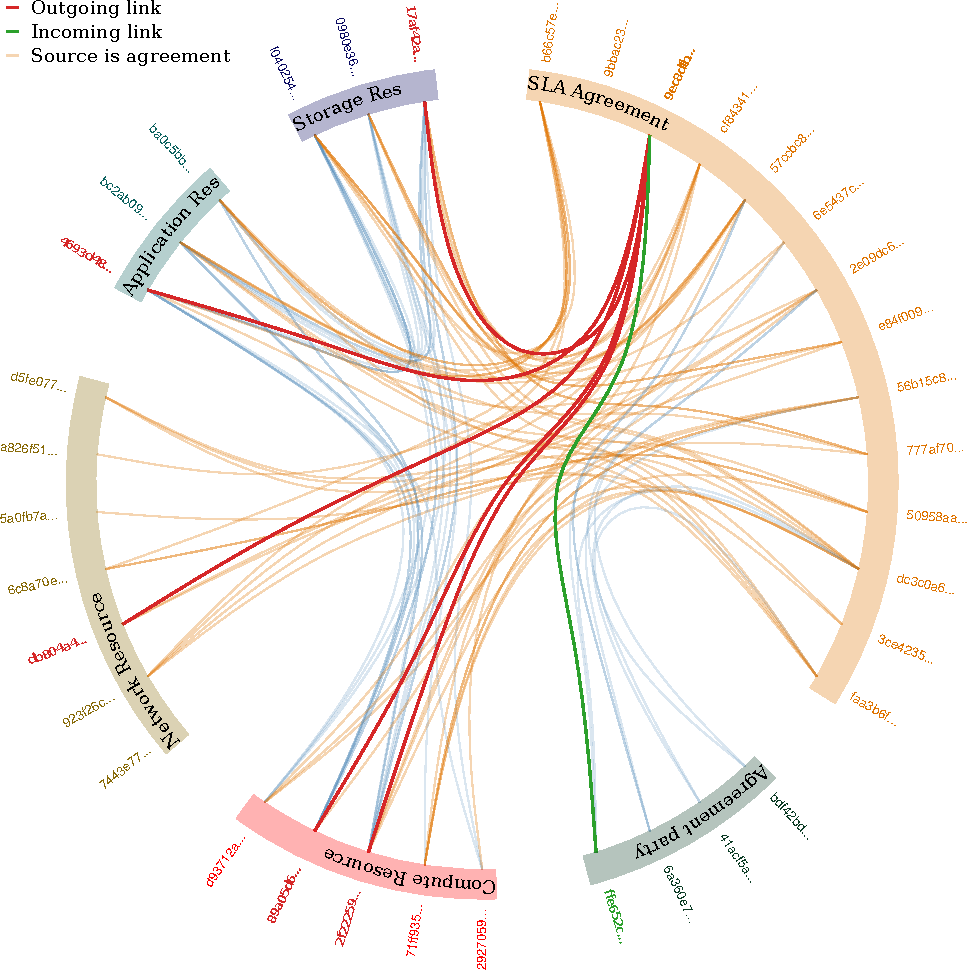
\includegraphics[width=0.9\textwidth]{images/occi.pdf}
		\caption{\emph{OCCI} verknüpft Dienstgüte-Vereinbarungen mit verteilten Anwendungen, Stakeholdern und Cloud-Ressourcen. Die Zuordnung erfolgt Service-bezogen. In der Abbildung ist eine Vereinbarung markiert: Sie wird von einem Anwender beantragt (grüne Linie) und wirkt anschließend auf Ressourcen und darauf aufbauenden Anwendungen (rote Linien). Visualisierung über \emph{OCCIViz}\protect\footnotemark.}	
		\label{fig:occi}
	\end{figure}

	\footnotetext{\url{https://github.com/IntelLabsEurope/OCCIViz}}
	
	Auch hier existiert eine experimentelle Implementierung für OpenStack\footnote{\url{https://github.com/openstack/ooi}}. Diese ist jedoch bereits als obsolet gekennzeichnet. Die SLA-Unterstützung ist über ein weiteres Projekt theoretisch verfügbar\footnote{\url{https://github.com/IntelLabsEurope/OCCI-SLAs}}.
	
	\emph{TOSCA} und \emph{OCCI} überschneiden sich nicht: Letzteres dient nicht der Modellierung providerübergreifender Infrastrukturen, sondern ausschließlich der Kommunikation mit der Plattform. Beide Standards ergänzen sich außerdem mit dem \emph{Cloud Data Management Interface (CDMI\footnote{\url{https://www.snia.org/cloud}})} für Verwaltung und Zugriff auf Netzwerkspeicher \cite{snia:2015:cdmi}. Konzeptionell wurden die Standards bereits zu einem modellbasierten Cloud-Orchestrationstool verbunden \cite{korte:2017:toscamp, carrasco:2018:toscamp}.
	%Model Driven Cloud Orchestration by Combining TOSCA and OCCI (Position Paper)
	%Fabian Korte, Johannes Martin Erbel, Jens Grabowski
	
	Um sinnvoll nutzbar zu sein, müsste der offene API-Standard von Cloud-Providern implementiert werden. Da dies nicht absehbar ist, bleibt \emph{OCCI} zumindest als interessante Grundlage für die API einer eigenen Cloud-Management-Plattform. Als pragmatischer Ersatz für den Zugriff auf Public-Cloud-Angebote, muss der Einsatz einer Multi-Cloud-Bibliothek evaluiert werden, siehe \autoref{sec:bibliotheken}.		
	
\end{description}

\noindent
Container sind nicht für jede Anwendung einsetzbar. Entsprechend müssen auch klassische virtuelle Maschinen bei einer Multi-Cloud-Migration unterstützt werden. Proprietäre Lösungen sind genauso ungeeignet wie Teillösungen auf einer einzelnen Service-Ebene.

Insgesamt ist der Support für offene Standards im Open-Source-IaaS-Projekt OpenStack am größten. Auf allen Ebenen der Service-Bereitstellung sind zumindest experimentelle Implementierungen verfügbar: \emph{cloud-init} zur Imagekonfiguration, \emph{TOSCA} zur Service-Definition und \emph{OCCI} zur Kommunikation mit der Cloud unter Berücksichtigung von SLAs. 

Einige weitere technische Herausforderungen löst ein Multi-Cloud-Broker oder eine CMP: Management von statischen und virtuellen IPs, SSL-Zertifikaten, sowie Load-Balancing. Andere Migrationshürden bleiben: Verfügbarkeit von Betriebssystemen, Frameworks und Bibliotheken, ebenso wie die Vereinbarkeit mit vorhandenen Lizenzen. Der folgende Abschnitt gibt eine Übersicht kommerzieller Cloud-Management-Plattformen sowie bisheriger Forschung zu Inter- und Multi-Cloud-Brokern mit besonderem Blick auf SLAs und Policys. 

\section{Die Limitierungen Kommerzieller CMPs}

Kommerzielle Anbieter wie \emph{RightScale} betonen den Self-Service-Charakter und potenzielle Kosteneinsparungen durch ihre Cloud-Management-Lösungen: Traditionell werden virtuelle Maschinen bei Bedarf von der internen IT bereitgestellt. Dabei entstehen auf der einen Seite Wartezeiten und auf der anderen erhöhter Arbeitsaufwand.

Eine CMP kann diese Arbeiten automatisieren. Sie helfe laut \emph{Rightscale} die \emph{Schatten-IT} abzubauen -- die entsteht, wenn Mitarbeiter aufgrund langwieriger interner Prozesse zu Public-Cloud-Angeboten greifen -- mit allen negativen Folgen für Sicherheit und Vertraulichkeit. Die automatische Durchsetzung von Policys könnte sich also doppelt lohnen. Nebenbei liefert die CMP einen Preis- und Feature-Überblick der internen und öffentlichen Angebote. So hilft sie, das optimale Angebot zu finden.

Nichtsdestotrotz sollte die CMP unabhängig entwickelt und betrieben werden. Cloud-Provider-eigene Lösungen werden daher nicht betrachtet. Weniger geeignet sind auch SaaS-Angebote: Hier entsteht eine neue Abhängigkeit und \emph{Single-Point-of-Failure}. Die nachfolgende Aufzählung zeigt die aktuell verbreitetsten CMP-Lösungen mit besonderem Fokus auf Bereitstellungsmodelle, Funktionsumfang und Offenheit der Schnittstellen.

\todo{(Zusatz) Tabelle OS + Kommerziell}

%Automatisierung oder nur schöne Dashboards?

\begin{description}
	
	\item[Red Hat CloudForms\footnotemark]\footnotetext{\url{https://www.redhat.com/en/technologies/management/cloudforms/}}
	Kommerzielle Cloud-Management-Plattform, Grundlage ist das Open Source-Projekt  \emph{ManageIQ}\footnotemark\footnotetext{\url{https://manageiq.org/}}, das alle wichtigen IaaS-Provider unterstützt (AWS, Azure, GCP, OpenStack).
	
	Besonderheit: ein umfangreiches -- optional grafisches -- Policy-Management. Eigene Regeln folgen dem Schema \emph{Bedingung/Ereignis-Aktion}.
	
	Alle Schnittstellen der CMP sind proprietär. Die Orchestrierung liest jedoch vorhandene Vorlagen aus \emph{AWS CloudFormation} and \emph{OpenStack Heat}.
	%http://manageiq.org/docs/reference/latest/doc-Policies_and_Profiles_Guide/miq/
	
	\item[Rightscale CMP\footnotemark]\footnotetext{\url{https://www.rightscale.com/}}
	Proprietäres \emph{Software-as-a-Service}-Angebot, unterstützt alle wichtigen IaaS-Provider, zusätzlich Plattformdienste, Docker-Container und Hypervisoren, besonders \emph{VMware vSphere}.
	
	Infrastruktur und Dienste werden als Vorlagen in einem eigenen Katalog bereitgestellt. Dabei erlaubt Rightscale auch heterogene Anwendungen über IaaS-, CaaS- und PaaS-Grenzen hinweg.
	
	Ein Dashboard zeigt Empfehlungen zur Kostenoptimierung, allerdings ohne SLAs einzubeziehen.
	
	\item[Scalr\footnotemark]\footnotetext{\url{https://www.scalr.com/}} war ursprünglich quelloffen unter GPL verfügbar. Diese Version wurde nach kurzer Ankündigung\footnote{\url{https://groups.google.com/forum/\#!topic/scalr-discuss/khFayhYJlhA}} im September 2017 innerhalb weniger Tage eingestellt. Seit dem existiert ausschließlich eine kommerzielle Closed-Source-Variante zum Betrieb auf eigener Hardware.	
	
	Verteilte Anwendungen werden mithilfe des \emph{Farm Builders} deklarativ in einer proprietären YAML-Datei beschrieben. Die Zuteilung von Cloud-Providern und Ressourcen ist explizit. Zusätzliche Regeln sind optional, werden aber nicht für ein Cloud-Brokering genutzt. Über einen internen Katalog können so beschriebene Anwendungen veröffentlicht werden.
	
	Die Policy-Unterstützung fokussiert sich auf Zugriffsrechte, Namenskonventionen, Kostenalarme und die Erfüllung bestimmter Audit-Anforderungen. Das Interface ist service- und anwenderbezogen. Dabei entsteht eine echte Abstraktion verschiedener Cloud-Infrastrukturen. Alle Funktionen sind jedoch nur für Amazon EC2 verfügbar.
	
	\item[Cloudify\footnotemark]\footnotetext{\url{https://cloudify.co/}} implementiert den \emph{TOSCA}-Standard und ist in einer Open-Source-Version erhältlich. Mithilfe (grafischer) Werkzeuge lassen sich Cloud-In\-fra\-struk\-tur\-en und Services modellieren. Plugins erweitern Cloudify um wichtige Provider; sowohl auf IaaS- (AWS, Azure, GCP, OpenStack) als auch auf CaaS-Ebene (Kubernetes). Konfiguration wie das Start-Skript kann direkt übergeben, oder über ein Tool wie Puppet weitergeleitet werden. 
	
	Einfache Policys sind integriert, mithilfe eines rudimentären Monitorings und der Provider-Plugins werden diese umgesetzt. Der (grafische) TOSCA-Editor und echtes Cluster-Management sind allerdings nur in der proprietären Enterprise-Ausgabe enthalten.


\end{description}

Die kommerziellen Cloud-Management-Plattformen fokussieren sich auf Kostenoptimierungen und Zugriffskontrolle. Portabilität von Anwendungen und Daten spielt aber nur eine untergeordnete Rolle. Ein Brokering auf SLA-Basis findet entgegen den Werbeversprechen nicht statt. Inwieweit Forschungsprojekte diese Lücke schließen können, prüft der nächste Abschnitt.

% https://www.embotics.com/solutions-cloud-governance
% Nur Azure und Amazon. Cloud Governance: Die richtigen Meta-Tags zu Instanzen hinzufügen. Kostenoptimierungsvorschläge, aber nur die Wahl zwischen zwei Providern.


%DivvyCloud (Commercial) 
%
%Automation Bots to schedule downtime, terminate, or re-size instances and resources so you only pay for what you use 
%
%https://divvycloud.com/product/botfactory/for-cost/ 

%
%Commercial Tools 
%
%https://www.cloudyn.com/ 
%
%close-source 
%
%only cost monitoring and optimization 
%
%Also, Cloudhealth, CloudCheckr 


\section{Bisherige Forschungsarbeiten}

Besonders interessant sind bisherige Arbeiten, die neben einer Föderation auch Hybrid- oder Multi-Cloud-Brokering unterstützen. Es sollten also keine Cloud-internen Plugins oder Agenten nötig sein.

Die folgende Übersicht geht besonders auf den Umfang der Policy- und SLA-Fähigkeiten ein: Diese sollten nicht nur während des Brokerings beachtet werden, sondern kontinuierlich zur Laufzeit. Auch die Einhaltung von Standards zu Service- und Ziel-Definitionen, sowie Kommunikation sind relevant. Unterschiede gibt es bei der Art unterstützter Anwendungen; neben Stapelverarbeitungsjobs und High-Performance-Computing sollten auch reguläre, interaktive Web-Anwendungen verwaltet werden können. 

Auch nicht-funktionale Anforderungen werden betrachtet: Sind die Artefakte der Projekte noch als Code verfügbar oder sogar in Open-Source-Tools und kommerziellen Produkten aufgegangen?

%policy-driven service placement optimization in federated clouds

\begin{description}	
	
	
	\item[InterCloud] ist ursprünglich eine Föderation von Cloud-Ressourcen \cite{buyya:2010:intercloud}. Auf einem zentralen Marktplatz \emph{zeigen} Clouds ihre Dienste, oder \emph{kaufen} sie je nach Bedarf. Für diese aktive Teilnahme sind Cloud-interne Agenten nötig.
	
	Vorgeschlagen werden zusätzlich externe Adapter, über die einerseits Provider \emph{unfreiwillig} in die Föderation integriert werden, andererseits aber auch weitere Teilnehmer Ressourcen kaufen können. Hierüber könnten auch Anwendungsbroker die Ressourcen der Föderation nutzen.
	
	Der Ansatz fokussiert sich stark auf das preisgesteuerte Brokering, beachtet optional aber auch Geostandorte. Die Provider unterstützen eingeschränkt SLAs. Verteilt werden nur Rechenaufgaben, interaktive Anwendungen sind nicht vorgesehen.
	%	5, 37, 38 Grozev	
	
	\item[Contrail] ist eine zentral gemanagte Föderation \cite{carlini:2011:contrail}. SLAs gelten für den gesamten Cloud-Verband, nicht für einzelne Anwendungen. Das zentrale Element, der \emph{Federation-Runtime-Manager}, verteilt jedoch individuelle Nutzeranfragen und beachtet dabei Preis und Leistung.
	
%	http://contrail-project.eu/architecture

	Contrail versteht sich als PaaS und unterstützt auch \emph{Hadoop}. Ähnlich zu \emph{InterCloud} sprechen externe Adapter theoretisch weitere Provider an, die sich der Föderation nicht bewusst sind.
			
	
	\item[RESERVOIR] entwickelt eine Peer-to-Peer-Föderation mit eigenen Service-Schemata und Inter-Cloud-Protokollen \cite{rochwerger:2009:reservoir}. Ein Unterprojekt abstrahiert die Cloud-Ressourcen durch eine zusätzliche Schicht, sodass Java-Anwendungen transparent auf allen Providern ausgeführt und migriert werden können \cite{rochwerger:2011:reservoir-multi-cloud}. Ein Broker beobachtet Performance-SLAs und skaliert die Instanzen entsprechend.
%	IBM, Telefonica, SAP + Universites, EU-funded
	
	
	\item[Optimis] baut auf eine zentrale \emph{Deployment Engine (DE)} \cite{ferrer:2012:optimis}. Über interne und externe Adapter verbinden sich Cloud-Provider und senden ihre Ressourcen-Angebote. Soll eine Anwendung ausgerollt werden, wählt die DE passende Provider aus und sendet ihnen ein SLA-Template. Diese antworten mit einer Zusage, Absage oder einem Gegenvorschlag. Aus allen Antworten wählt der DE anschließend das beste Angebot. Dabei beachtet sie quantitative Größen wie den Preis, aber auch Erfahrungswerte wie Zuverlässigkeit oder die Energieeffizienz eines Providers.
	
	Die internen Adapter vertreten Föderationsmitglieder -- sie lehnen eine Anfrage des DE ab, wenn sie für den Cloud-Provider finanziell unattraktiv ist. Eine weitere Komponente, der \emph{Service-Optimizer}, beobachtet alle Anwendungen auf SLA-Verletzungen. Wie genau SLAs spezifiziert werden können, ist nicht deutlich. Auch der Matching-Algorithmus ist nicht öffentlich. Geostandorte werden nicht beachtet. Externe Adapter sind rein konzeptionell und nicht implementiert.
	
	Die Arbeit geht auch auf die Bereitstellung von Laufzeitumgebungen und Provider-spezifischen Images ein: Er schlägt eine Erweiterung des \emph{Open Virtualization Formats (OVF)} vor. Zusätzliche Metadaten beschreiben die nötige Cloud-Konfiguration.
	
	
	\item[Bernsetein InterCloud Blueprint] Eine weltweite Föderation der Cloud-Ressourcen \cite{bernstein:2011:intercloud}. Interessant ist der dezentrale Ansatz des Brokerings. Nur in dieser Arbeit wird der Broker als \emph{Single-Point-of-Failure} erkannt: Deshalb soll er zwangsläufig repliziert und in allen Regionen mindestens einmal verfügbar sein. Der Ansatz folgt also den Grundlagen des Internets und entwickelt eigene Inter-Cloud-Protokolle auf Basis von XMPP und RDF.
	
	
	\item[STRATOS] ist eine Cloud-Management-Plattform mit integriertem Multi-Cloud-Broker \cite{pawluk:2012:stratos}. Anwendungen werden über das eigenentwickelte, XML-basierte \emph{Topology Descriptor File (TDF)} beschrieben. Es enthält die Service-Architektur und zusätzlich Policys und SLOs. Für den Zugriff auf externe Clouds existiert ein \emph{Translation-Layer}, der eine einheitliche API bereitstellt. Die Arbeit fokussiert sich auf die Bereitstellung klassischer Web-Anwendungen und Kostenoptimierung. Der mittlerweile nicht mehr weiterentwickelte \emph{Service Measurement Index (SMI)} definiert die Ziele.
%	https://www.google.de/url?sa=t&rct=j&q=&esrc=s&source=web&cd=1&ved=0ahUKEwju27vHs6DZAhUCWRQKHRv7BEcQFggrMAA&url=http%3A%2F%2Fwww.mikesmit.com%2Fwp-content%2Fpapercite-data%2Fpdf%2Fcloud2012.pdf&usg=AOvVaw3e6yhHYmhWBbIxtr7MqkuX
	
	\item[Meryn] ist eines der wenigen Implementierung eines SLA-bezogenen PaaS-Systems \cite{dib:2013:meryn}. Aktuelle Plattformen begrenzen hauptsächlich den Ressourcenverbrauch der Gastanwendungen -- Meryn schlägt zusätzlich eine Kostenoptimierung für Provider vor.
	
	Cloud-interne \emph{Cluster-Manager} bieten in einem Wettbewerb um Ausführungsaufträge. Die Arbeit fokussiert sich auf Stapelverarbeitung mit Hadoop und anderen Framworks. Dabei entwickeln die Autoren für jedes Framework eine eigene VM, die jeweils einmal pro Cluster ausgeführt wird. Vorgestellt wird außerdem ein \emph{Cloud-Bursting-Ansatz}, bei dem zusätzliche Ressourcen in Public Clouds angemietet werden.
	
	
	\item[SeaClouds] ist ein EU-finanziertes PaaS-Management-Projekt mit großem Umfang \cite{seaclouds:2015:architecture}. Vorgeschlagen wir ein Referenzmodell aus \emph{Planner}, \emph{Deployer}, \emph{SLA-Service} und \emph{Monitor}. Hierüber lassen sich verteilte Anwendungen modellieren, auf verschiedenen Providern bereitstellen und SLA-bezogen verwalten.
	
	Besonderheit ist die Unterstützung von offenen Standards wie der \emph{Cloud Application Management for Platforms (CAMP)} für APIs und TOSCA zur Service-Modellierung. Angebote der Cloud-Provider werden kontinuierlich überwacht und als \emph{TOSCA}-Graph abgebildet. SLAs nutzen allerdings nicht \emph{TOSCA}, sondern \emph{WS-Agreements}.
%	http://wsag4j.sourceforge.net/site/wsag/wsag-language.html
		
	Erwähnt wird eine Provider-unabhängige Lösung, konkret umgesetzt ist dies jedoch nur für die Open-Source-PaaS-Projekte \emph{OpenShift} und \emph{CloudFoundry}.
	
	\item[TOSCAMP] oder \emph{End-to-End Orchestration of
	Multi-Cloud Applications}, kombiniert in einem Prototyp die Standards \emph{TOSCA} und \emph{CAMP} \cite{korte:2017:toscamp}. Eine verteilte Anwendung wird abstrakt als \emph{TOSCA}-Template inklusive einfacher Policys beschrieben. Anschließend wandelt \emph{TOSCAMP} diese Beschreibung in einen \emph{CAMP}-Plan zur Multi-Cloud-Installation.

	Im Gegensatz zu anderen Cloud-Management-Plattformen erstellt \emph{TOSCAMP} keinen internen Graphen einer Anwendung -- stattdessen erweitert die Arbeit \emph{CAMP} um Policys und bildet alle Installationen in einer YAML-Datei ab. Einen ähnlichen Ansatz verfolgt das Projekt \emph{brooklyn-tosca\footnote{\url{https://github.com/cloudsoft/brooklyn-tosca}}}.
	
%	\item[An SLA-based Broker for Cloud Infrastructures] Nicht nur Private Clouds sondern auch Personal Devices 
%	
%	Modulare Architektur 
%	
%	wechselnde und unzuverlässige Provider
%	
%	Fokus auf Föderation. Aber: Idee der forced integration of commercial cloud providers 
	
\end{description}

%Mist.io Open source 
%Build on libcloud and cloudify
%Can monitor costs (commercial)
%No automatic scheduling 

\noindent
Im Gegensatz zu den kommerziellen Projekten liegt der Fokus vieler Forschungsarbeiten auf Cloud-Föderationen und SLA-basiertem Brokering. Einige unterstützen über Adapter konzeptionell mehrere Bereitstellungsmodelle; je nachdem, ob dem Cloud-Provider die Mitgliedschaft in einer Föderation bewusst ist. Interne Adapter sprechen mit zusätzlichen, Cloud-internen Erweiterungen. Externe Adapter nutzen die öffentlichen APIs von Drittanbieter-Clouds. Hier entsteht zwar Mehraufwand, dieser könnte in weiteren Entwicklungen jedoch von einer Multi-Cloud-Bibliothek gemildert werden.

Negativ fällt auf, dass die Artefakte der meisten (EU-)Forschungsprojekte
nicht mehr verfügbar sind \cite{blasi:2013:eu-projects-overview}. Auch Matching-Algorithmen sind teilweise nicht veröffentlicht. Die Ergebnisse lassen sich so nicht mehr nachvollziehen. Ohnehin basieren sie oft auf veralteten Technologien: Formate wie \emph{OVF} werden in modernen IaaS-Plattformen nicht mehr unterstützt. Demgegenüber spielen Container oder Serverless-Computing keine Rolle.

Wie bereits beschrieben, existieren eine Vielzahl von offenen Cloud-Standards \cite{bmwi:2012:cloud-standards}. Von Service-Definition über SLAs bis zur standardisierten Kommunikation mit der Management Plattform. In der Forschung werden diese aber nur selten aufgegriffen und stattdessen neu erfunden. Besonders deutlich wird die in einer Forschungsübersicht der Europäischen Kommission.
%Cloud Computing Service Level
%Agreements
%Exploitation of Research Results
%Editor: Dimosthenis Kyriazis
Das eigentliche Problem der Portabilität im Cloud-Umfeld lässt sich so nicht lösen.

Insgesamt bleibt vor allem die unterschiedliche Ausrichtung von Forschungsprojekten und kommerziellen Anbietern: Forschungsprojekte fokussieren sich auf Föderationen. Dies entspricht auch dem vorherrschenden Cloud-Typ innerhalb der verantwortlichen Organisationen. SLAs werden ausschließlich von diesen ausgewertet und teilweise umgesetzt. Kommerzielle Projekte sind dagegen meist externe Broker, stellen Preisunterschiede und Kosten dar. Statt SLAs beachten sie nur einfache Policys.

Das folgende Kapitel erstellt aus den bisherigen Überlegungen zu Anforderungen, Schemata und Forschungsergebnissen einen Vorschlag für SLA-basiertes Brokering auf Basis moderner Technologien.

	\chapter{Entwurf und Implementierung}
\label{cha:implementierung}

\todo{Kapitel-Einleitung}



\section{Modularer Architektur-Vorschlag}

%Komponenten des Brokers.
%
%
%In der CMP: Polling oder Notification?
%
%Was löst eine Aktion aus?
%- Monitoring der Services
%- Änderung der Umgebung
%- User-Aktion
%- Ergebnis einer anderen Policy

\begin{figure}
	\centering	
%	\def\svgwidth{0.95\textwidth}
%	{\tiny
%	\includesvg{images/broker-cycle}}
	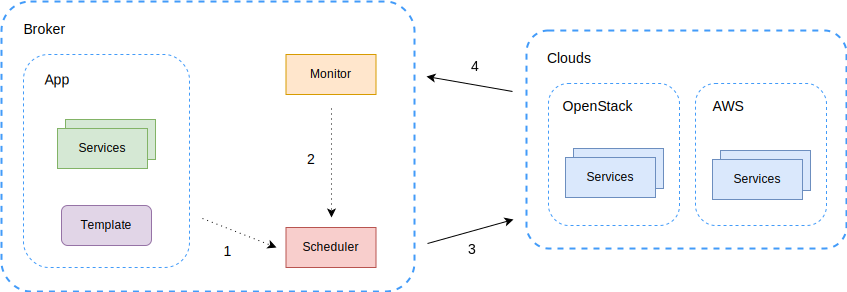
\includegraphics[width=\linewidth]{images/broker-cycle}
	\caption{Arbeitsweise des Multi-Cloud-Brokers als Zyklus: (1) Sammeln der Meta-Informationen aller Cloud-Provider, (2) Sammeln der Laufzeitinformationen der Anwendungen, (3) Sammeln der SLAs, (4) Nutzeränderungen: Neue Anwendungen oder Anpassung von SLAs, (5) Optimierungsplanung, (6) Planausführung auf den Cloud-Infrastrukturen}
	\label{fig:cycle}
\end{figure}

%Zyklus\autoref{fig:cycle}:

%\begin{description}
%	\item[Nummerierte Aufzählung]~\par
\begin{enumerate}
	
	\item Sammeln der Meta-Informationen alle Cloud-Provider
	\begin{enumerate}
		\item Kapazität (CPU, RAM, HDD, Network)
		\item Features (Verschlüsselung, CUDA, …)
		\item Geo-Lokation 
		\item Preis
	\end{enumerate}
	
	\item Sammeln der Laufzeitinformationen der PaaS/Anwendungen
	\begin{enumerate}
		\item Auslastung
		\item Fehler
		\item Ausfälle
	\end{enumerate}
	
	\item Sammeln der SLAs
	\begin{enumerate}
		\item Policy-Definitionen
		\item Policy-Konfiguration
		\item Placement-Algorithmen
	\end{enumerate}
	
	\item Neue Anwendung/Änderung eines SLA
	
	\item Optimierung
	\begin{enumerate}
		\item Feste Vorgaben (Geo, Backup)
		\item Weiche (Preis, Latenz, Verfügbarkeit)
	\end{enumerate}
	
	
	\item Ausführung
	\begin{enumerate}
		\item Netzwerkkonfiguration
		\item Allokation/De-Allokation von Ressourcen
		\item Deployment
		\item Migration
		\item Logging/Benachrichtigung
		\item Backup
	\end{enumerate}
	
\end{enumerate}

\section{Brokering}


%https://de.wikipedia.org/wiki/Constraintprogrammierung
%https://de.wikipedia.org/wiki/Scheduling

%entailing multiple constraint satisfaction (MCS)
%
%\todo{Schaubild, was wird wann gematcht}
%% Pseudocode des Algorithmus, wie in Meryn
%
%Kostenoptimierung
%
%Preisentwicklung? 
%
%Migration je nach Tageszeit? 
%
%Kosten der Datentransfers 
%
%Subscription On-Demand/Monthly/Yearly 
%
%Kompliziert durch undurchsichtige Staffelpreise
% https://www.rightscale.com/blog/cloud-cost-analysis/aws-vs-azure-vs-google-cloud-pricing-compute-instances

%https://www.rightscale.com/blog/cloud-cost-analysis/comparing-cloud-instance-pricing-aws-vs-azure-vs-google-vs-ibm

%
%Cost Calculators 
%
%http://go.appscale.com/cloud-cost-calculator-help 
%
%https://github.com/ifosch/accloudtant 
%
%https://awstcocalculator.com/# 
%

\section{Testanwendung: Hyrise-R}

Hyrise\footnote{\url{https://hpi.de/plattner/projects/hyrise.html}} ist eine In-Memory-Forschungsdatenbank der Fachgruppe \emph{Enterprise Platform and Integration Concepts (EPIC)} am Hasso-Plattner-Institut \cite{grund:2010:hyrise}. Die Datenbank teilt sich einige Eigenschaften mit \emph{SAP HANA}\footnote{\url{https://www.sap.com/products/hana.html}}: Ein \emph{Delta Store}, spaltenorientierte Speicherung, Wörterbuchkodierung und weitere Komprimierungstechniken sowie den \emph{Insert-Only}-Ansatz und Partitionierung. Herausragend ist die OLAP-Performance, enthalten sind aber auch Optimierungen für OLTP-Aufgaben.

Hyrise-R ist eine Erweiterung des Basisprojektes um Replikation \cite{schwalb:2015:hyrise-r}. Es folgt dabei dem \emph{Scale-Out}-Ansatz: Alle schreibenden Operationen werden auf einem einzigen \emph{Master-Node} durchgeführt. Dessen Datensatz wird in weniger als einer Sekunde (\emph{lazy}) mit beliebig vielen \emph{Replica-Nodes} abgeglichen. Diese Spiegelungen bearbeiten alle reinen Leseanfragen und machen den Verbund so skalierbar, siehe \autoref{fig:hyrise-r}. Nach dem \emph{CAP-Theorem} sind Verfügbarkeit und Partitionstoleranz hier also wichtiger als Konsistenz. 

\begin{figure}[ht]
	\centering
	\def\svgwidth{0.9\textwidth}
	\textsf{
	\includesvg{images/hyrise-r}}
	\caption{Verteilte \emph{Hyrise-R}-Architektur mit getrennter Verarbeitung von Lese- und Schreibanfragen. Der Master-Knoten dient als \emph{Single Source of Truth}. Zur Leistungssteigerung übernehmen Spiegelserver die Beantwortung der meisten Leseanfragen. Kleinere Inkonsistenzen werden dabei in Kauf genommen. Nicht im Bild ist der Dispatcher zur Anfrageverteilung. Aus \cite{ssiclops:d42:experiments-measurements}.}	
	\label{fig:hyrise-r}
\end{figure}

Durch die verteilte Architektur ist Hyrise-R ein potenzieller Kandidat als Testanwendung innerhalb der Multi-Cloud-Umgebung. Einige \emph{SSICLOPS}-Teilprojekte untersuchten bereits Zuverlässigkeit, Performance, Datensicherheit und Vertraulichkeit in einer privaten OpenStack-Föderation \cite{ssiclops:d23:security-extensions, ssiclops:d42:experiments-measurements, bastian:2017:openstack-policies}. \todo{Diagramm:Hyrise-R on OS}

Im Rahmen dieser Arbeiten sind einige Infrastrukturteile als Code veröffentlicht: So existiert zum Beispiel eine Docker-Teststellung mit grafischem Cluster-Manager, um die Performance bei verschiedenen Replikationsstufen zu prüfen. Diese Infrastruktur wurde in mehreren Studienarbeiten weiter angepasst, um Hyrise-R-KVM-Images in OpenStack bereitzustellen \cite{eschrig:2016:ssiclops-masterproject, maschler:2017:ssiclops-masterproject}.

Um als Testanwendung über mehrere Cloud-Ebenen zu dienen, sollte Hyrise-R auf den verbreiteten Hypervisoren, IaaS- und CaaS-Providern ausführbar sein. Aufgrund der Softwarestruktur -- als eigenentwickelte \emph{Low-Level-C++-Anwendung} --  eignet Hyrise-R sich nicht direkt\footnote{\url{https://cloud.google.com/appengine/docs/flexible/custom-runtimes/}} als Testanwendung für die PaaS-Integration. Hierfür nutzen wir andere Standardsoftware, die auf den üblichen PaaS-Sprachen wie Java, Python oder Node.js aufbauen.

Hyrise-R ist von Anfang an für die Skalierung über externe Broker konzeptioniert. Die bisherigen Arbeiten haben \emph{Standalone-Cluster-Manager} umgesetzt, erst für Docker und später für OpenStack\footnote{\url{https://github.com/DukeHarris/hyrise_rcm}}\footnote{\url{https://github.com/SSICLOPS/openstack-testbed-vm}}. Die nötigen Clusterinformationen werden Hyrise-Instanzen direkt beim Start als Parameter übergeben. Variablen zur Laufzeitumgebung müssen während des Deployments vom Broker ausgefüllt werden: Konkret benötigt Hyrise einen TCP-Port und eine eindeutige Knoten-ID. Über ihre ID registrieren sich Knoten am Dispatcher. Hierzu benötigen sie dessen IP-Adresse und Port -- der Dispatcher muss also immer als Erstes in einem Cluster bereitstehen. Erst dann können Start und Registrierung des Masters erfolgen. Plattformunabhängig ergeben sich folgende Startskripte für einen Hyrise-R-Cluster:

\begin{description}
	
\item[{[1]} Dispatcher] einmal pro Cluster, zentrale Lastverteilung für alle Anfragen
	
\begin{minted}{jinja}
./dispatcher {{dispatcher.port}} settings.json
\end{minted}
	
\item[{[1]} Master] einmal pro Cluster als \emph{Single-Source-of-Truth}, bearbeitet alle Schreibanfragen, gekennzeichnet durch \emph{nodeId=0}
	
\begin{minted}{jinja}
./hyrise \
  --dispatcherurl={{dispatcher.ip}} \
  --dispatcherport={{dispatcher.port}} \
  --nodeId=0 \
  --port={{master.port}}
\end{minted}

\item[{[0-n]} Replica] optional, beliebig viele Instanzen pro Cluster zur Entlastung des Master-Knotens bei Leseanfragen

\begin{minted}{jinja}
./hyrise \
  --dispatcherurl={{dispatcher.ip}} \
  --dispatcherport={{dispatcher.port}} \
  --nodeId={{replica.id}} \
  --port={{replica.port}}
\end{minted}
	
\end{description}

\noindent
In vorherigen Projekten entwickelte Images für virtuelle Maschinen laufen auf der verbreiteten Hypervisorkombination aus QEMU und KVM. Die Erstkonfiguration erfolgte bisher über direkte SSH-Kommandos an die gestartete virtuelle Maschine. Dies erfordert die Konfiguration von SSH in den VMs und die Verwaltung von Schlüsseln in der CMP. Zusätzlich entsteht eine Wartezeit zwischen VM-Startkommando und Erstkonfiguration, die vorherige Projekte durch Polling noch ausdehnten. Eine elegantere Lösung ist \emph{cloud-init}: Die CMP füllt ein Konfigurationstemplate und schickt es direkt im Startkommando an den Infrastruktur-Provider. Dieser führt das Skript sofort ohne weitere Wartezeit aus.

Auch Docker-Images existieren bereits\footnote{\url{https://github.com/hyrise/hyrise-v1/tree/feature/docker}}, wurden aber seit 2015 nicht aktualisiert: Docker, diverse Abhängigkeiten und Hyrise selbst wurden in der Zwischenzeit weiterentwickelt. Innerhalb eines Clusters sollten alle Knoten dieselbe Hyrise-Version ausführen. Daher aktualisieren wir Dispatcher und Hyrise auf Basis des aktuellsten Hyrise-NVM-Branches\footnote{\url{https://github.com/janmattfeld/dispatcher/tree/docker}}\footnote{\url{https://github.com/janmattfeld/hyrise_nvm/tree/feature/docker}}.

Die Aktualisierung enthält das aktuelle Docker-Basis-Image Ubuntu 16.04. Wir integrieren außerdem korrekte Metadaten und Dokumentation zur Imageerstellung und Ausführung. Einige eingebundene Git-Submodule wurden in der Zwischenzeit verschoben oder existieren nicht mehr -- die verwendete CSV-Bibliothek muss zum Beispiel ausgetauscht werden. Dies erfordert kleinere Änderungen am Quellcode. Genauso wie neue \emph{Non-Uniform-Memory-Access-Funktionen (NUMA)}: Die Funktion \emph{membind} erfordert erweitere Rechte. In einem Standard-Docker-Container sind diese aber nicht vorhanden. Der neue Startparameter \mbox{\emph{-\,-disable\_membind}} deaktiviert die speziellen NUMA-Funktionen. Unsere Images laufen daher auch in Container-Laufzeitumgebungen der Public-Cloud-Provider.

Das Image ist zum Produktivbetrieb gedacht: Docker Build entfernt nach dem Image-Erstellungsprozess alle Abhängigkeiten, die zum Betrieb nicht notwendig sind. So reduziert sich die Image-Größe von über 500 auf weniger als 300\,MB -- entsprechend verkürzt sich die Startzeit. Enthalten ist außerdem eine Beispieldatenbank, die wir später als Benchmark und initialen Funktionstest nutzen werden. Gemessen wird also nicht die Synchronisationszeit der Hyrise-R-Lösung, sondern die Skalierungsfähigkeiten der verwendeten Cloud-Lösungen und Orchestrierungstechniken. Wir setzen außerdem pragmatische Startparameter für Hyrise-R auf Docker: \emph{-\,-corecount=2} \emph{-\,-disable\_membind}. Die neuen Images sind zur leichteren Integration auf Docker Hub veröffentlicht\footnote{\url{https://hub.docker.com/r/hyrise/dispatcher/}}\footnote{\url{https://hub.docker.com/r/janmattfeld/hyrise_r/}}. Um auch zukünftige Weiterentwicklungen von Hyrise nutzen zu können, automatisiert ein neues Makefile Docker-Build-Voränge und den Realease auf Docker Hub.

Aus der bisher losen Sammlung von Quellcode, Shell-Skripten und Makefiles in mehreren GitHub-Repositorys haben wir eine nachhaltige Pipeline zur automatisierten Image-Erstellung für verschiedene Infrastrukturen entwickelt\footnote{\url{https://github.com/janmattfeld/hyrise_nvm/commit/cfe3aa8}}. Ausführungsumgebung, Programm, Testdaten und Konfiguration werden flexibel integriert -- Hyrise-R eignet sich nun als Testanwendung für den Multi-Cloud-Broker.

Als Weiterentwicklung zu den bisherigen Hyrise-R-Arbeiten soll der Broker nicht nur nach Leistungsanforderungen skalieren, sondern auch SLAs und Geostandorte beachten sowie diverse Infrastrukturanbieter nutzen.


\section{Private-Cloud: OpenStack-Testbed}

Als Beispiel für eine Private-Cloud -- als Teil unseres Multi-Cloud-Setups -- soll OpenStack dienen. Es ist das populärste Open-Source-Projekt um eigene Infrastruktur als Service aufzubauen. Gesponsert wird es von Großunternehmen wie \emph{HPE}, \emph{IBM}, \emph{Canonical}, \emph{Red Hat} und anderen.

OpenStack setzt sich aus verschiedenen Teilprojekten zusammen, die jeweils einen Dienst entwickeln und bereitstellen. Ein Minimal-Setup besteht aus \emph{Nova} (Computing), \emph{Key\-stone} (Authentifizierung), \emph{Neutron} (Netzwerk) und \emph{Glance} (Images). Verbreitet sind außerdem \emph{Cinder} (Blockspeicher) und \emph{Horizon} (Dash\-board). Diese sollen auch in unserem Beispiel genutzt werden. Denkbar ist darüber hinaus die Integration eines Container-Dienstes. Der Zugriff auf die Infrastruktur erfolgt entweder über das Dashboard, Kommandozeilentools oder eine REST-API.

Grundsätzlich wäre auch der Aufbau einer OpenStack-Föderation wie in \emph{SSICLOPS} denkbar \cite{ssiclops:2015:d6.1-project-presentation}. Föderierte Cloud-Architekturen teilen sich zentrale Komponenten, in OpenStack mindestens den Authentifizierungsservice \emph{Keystone}. Je nach Föderationsvariante (\emph{Cells}, \emph{Regions}, \emph{Availability Zones} oder \emph{Host Aggregates}) sind auch Dienste wie Dashboard oder Speicher nur einmal vorhanden. Diese Architektur reduziert Fixkosten, erfordert allerdings spezielle Anpassungen innerhalb der Cloud. Auch gehen einige Vorteile wie Ausfallsicherheit und Unabhängigkeit der zentralen Dienste wieder verloren. Eine Kombination mit weiteren Cloud-Providern im Rahmen unseres Multi-Cloud-Setups ist denkbar, bleibt aufgrund der aufwendigen Einrichtung aber außen vor. Auch wäre der zusätzliche Erkenntnisgewinn vermutlich gering.\todo{SSICLOPS-OS-Architektur}

Selbst ein minimales OpenStack-Testsetup ist durch die diversen Dienste komplex. Denkbar wäre also auch die Nutzung von externen OpenStack-Angeboten. In diesem Projekt gibt es hierfür grundsätzlich drei mögliche Bereitstellungsmodelle: 

\begin{enumerate}
	\item Public Cloud
	\\\emph{Betrieb auf geteilter Cloud-Infrastruktur}
	
	\item Hosted Private Cloud
	\\\emph{Betrieb auf exklusiver Cloud-Infrastruktur}
	
	\item Lokale Testinstallation
	\\\emph{Betrieb auf eigener physischer oder virtueller Infrastruktur}
\end{enumerate}

\noindent Eine Liste öffentlicher OpenStack-Angebote findet sich auf der Projekthomepage\footnote{\url{https://www.openstack.org/marketplace/hosted-private-clouds/}}. Dort werden auch weitere Informationen wie Funktionsumfang und Zertifizierungen aufgeführt. 

Interessant ist zum Beispiel das Angebot der Deutschen Telekom \emph{Open Telekom Cloud\footnote{\url{https://cloud.telekom.de/en/infrastructure/open-telekom-cloud/}}}: eine Public Cloud auf OpenStack-Basis -- in Deutschland -- mit vollem Funktionsumfang und API-Zugriff. International bietet \emph{Rackspace} eine Hosted Private Cloud\footnote{\url{https://www.rackspace.com/openstack/}}. Beide eignen sich jedoch kaum, um kleine Experimente zu starten, sondern richten sich vor allem preislich an größere Organisationen und Unternehmen.

Kostenlos ist das Public-Cloud-Angebot \emph{TryStack}\footnote{\url{http://trystack.org/}}. Sponsoren wie \emph{Cisco}, \emph{NetApp}, \emph{Dell} und \emph{Red Hat} finanzieren das Projekt. Die Registrierung erfolgt über die Aufnahme in eine Facebook-Gruppe, anschließend soll hierüber auch der Zugang zur kostenlosen OpenStack-\emph{Liberty}-Instanz erfolgen. Während der gesamten Laufzeit dieser Arbeit war allerdings weder ein Login noch Kontakt zu den Organisatoren möglich.

Lokale OpenStack-Installationen sind aufwendig: Für jeden Dienst muss ein eigener physikalischer Rechner bereitstehen. Dementsprechend verweist die offizielle Dokumentation direkt auf die Vielzahl von OpenStack-Distributionen\footnote{\url{https://www.openstack.org/marketplace/distros/}}. Diese bieten fast immer einen vereinfachten Setup-Prozess und oft die Option statt physikalischen Rechnern virtuelle Maschinen oder Container zu nutzen. Wie auch bei den Hosted-Angeboten sind hier nicht alle Dienste verfügbar. In allen Paketen fehlt \emph{Zun}, der aktuelle Container-Service.

Speziell für lokale Test- und Entwicklungsumgebungen existiert \emph{DevStack}\footnote{\url{https://docs.openstack.org/devstack/latest/}}. Das offizielle OpenStack-Projekt installiert automatisiert die wichtigsten OpenStack-Dienste auf einer einzigen Maschine. Ausdrücklich unterstützt werden dabei auch VMs und \emph{LXC}-Container. Es soll daher als Erstes erprobt werden.

\section{DevStack virtualisiert inkl. Container-Support}

Während der Installation nimmt DevStack tief greifende Veränderungen am Hostsystem vor. Es müsste also auf einem separaten Server installiert werden. Dieser Abschnitt beschreibt den Versuch einer virtualisierten, reproduzierbaren DevStack-Testinstallation. Außerdem soll \emph{Zun} integriert werden. 

Ziel ist DevStack in einem Container auszuführen, genauso wie die darin gestarteten Compute-Nodes ebenso in einem -- nun verschachtelten -- Container bereitzustellen. Die Gründe hierfür sind zusammengefasst:

\begin{enumerate}
	\item Keine oder minimale Änderungen am Hostsystem
	\item Reproduzierbarer Testaufbau
	\item Schneller und rückstandsloser Reset
	\item Zustände (\emph{Snapshots}) speicherbar
	\item Schnelle Ausführung von Gastapplikationen
\end{enumerate}

\noindent Auch eine virtuelle Maschine löst die oben genannten Probleme. Theoretisch. Problematisch wird die Ausführungsgeschwindigkeit von Gastanwendungen in einem mit \emph{VirtualBox} virtualisierten OpenStack. Eine Lösung ist \emph{verschachteltes KVM}, das bereits in der Arbeit [1] erprobt wurde. Die Autoren empfehlen ihren Vorschlag bei bestehenden Erfahrungen mit \emph{libvirt}. Der damalige Versuchsaufbau stellt sich allerdings als instabil und nicht mehr reproduzierbar heraus.

\begin{figure}[ht]
	\centering
	\begin{subfigure}[b]{0.29\textwidth}
		\def\svgwidth{\linewidth}
		{\tiny
			\includesvg{images/devstack-bare-metal}}	
		\caption{Bare-Metal-Installation}
		\label{fig:sub:devstack-bare-metal}
	\end{subfigure}\hfill%
	\begin{subfigure}[b]{0.31\textwidth}
		\def\svgwidth{\linewidth}
		{\tiny
			\includesvg{images/devstack-vm}}	
		\caption{All-in-One-VM}
		\label{fig:sub:devstack-vm}
	\end{subfigure}\hfill%
	\begin{subfigure}[b]{0.31\textwidth}
		\def\svgwidth{\linewidth}
		{\tiny
			\includesvg{images/devstack-docker}}	
		\caption{DevStack in Docker}
		\label{fig:sub:devstack-docker}
	\end{subfigure}
	
	\caption{Verschiedene Installationsvarianten für eine OpenStack-Testinstallation mit DevStack auf einem einzelnen Host -- inklusive Unterstützung für Docker-Compute-Container und klassische VMs. Eine direkte Installation verändert unwiderruflich das gesamte Host-System \emph{(a)}. Eine VM benötigt mehr Ressourcen und kann die Geschwindigkeit der Gastanwendungen negativ beeinflussen \emph{(b)}. Die Installation in einem Container schafft Abstraktion und Reproduzierbarkeit ohne Geschwindigkeitskompromisse. Die Gastcontainer nutzen weiterhin den Kernel des Host-OS \emph{(c)}.}
	\label{fig:devstack}
\end{figure}

\emph{LXD}-Container könnten sich ebenfalls eignen. Im Gegensatz zu Docker führen sie mehrere Prozesse aus, erinnern also mehr an eine klassische virtuelle Maschine (ohne deren Overhead). Laut Entwickler \emph{Canonical} fokussiert sich \emph{LXD} speziell auf IaaS-Aufgaben\footnote{\url{https://www.ubuntu.com/containers/lxd}}. Ein LXD-DevStack-Setup birgt allerdings die gleichen Hürden\footnote{\url{https://docs.openstack.org/devstack/latest/guides/lxc.html}} wie ein Docker-Setup \cite{graber:2016:openstack-lxd}. Beachtenswert ist noch das OpenStack-Projekt \emph{Kolla}, das jeden OpenStack-Dienst in einem eigenen Docker-Container installiert\footnote{\url{https://cloudbase.it/openstack-kolla-hyper-v/}}.

Um Container innerhalb von OpenStack auszuführen, gibt es mehrere, teils konkurrierende Projekte. Alle lassen sich über Plugins in DevStack einbinden. Dies sind die wichtigsten \cite{singh:2017:containers-openstack}:

\begin{description}
	
	\item[Zun\footnotemark]\footnotetext{\url{https://wiki.openstack.org/wiki/Zun}} Eigenständige OpenStack-API zum Starten und Verwalten von diversen Containertypen, inklusive \emph{Docker}.
	
	\item[Nova Docker\footnotemark]\footnotetext{\url{https://wiki.openstack.org/wiki/Docker}} Im Gegensatz zu \emph{Zun} erfolgt die Docker-Containerverwaltung über die bekannte Nova-API. Das Projekt wurde eingestellt.
	
	\item[Nova LXD\footnotemark]\footnotetext{\url{https://linuxcontainers.org/lxd/getting-started-openstack/}} Parallel zu \emph{Nova Docker} erfolgt der Zugriff über die Nova-API. Das Projekt wird von \emph{Canonical} aktiv vorangetrieben. Weiterer Teil ist die Automatisierung via \emph{Juju}.
	
	\item[Magnum\footnotemark]\footnotetext{\url{https://wiki.openstack.org/wiki/Magnum}} Eine Self-Service-Lösung zur Orchestrierung auf Basis von \emph{Heat}. Stellt automatisiert Container Orchestration Engines (COEs) wie \emph{Docker Swarm} und \emph{Kubernetes} bereit.
	
\end{description}

\noindent DevStack in Docker wurde bereits vor einiger Zeit umgesetzt\footnote{\url{https://github.com/ewindisch/dockenstack}}. Da das Projekt nicht mehr gepflegt wird und auf das ebenfalls beendete \emph{Nova Docker} aufsetzt, erfolgt die Neuimplementierung mit folgenden Änderungen:

\begin{itemize}
	
	\item Ubuntu-LTS-Basis-Image 14.04 $\Rightarrow$ 17.10
	\item Mehrprozessunterstützung per \emph{systemd}\footnote{\url{https://docs.openstack.org/devstack/latest/systemd.html}}
	\item OpenStack-Version Kilo $\Rightarrow$ Pike
	\item libvirt/QEMU-Instanzen
	\item Nova Docker $\Rightarrow$ Zun
	\item Container-angepasste DevStack-Konfiguration
	\item Vollständige Netzwerkkonfiguration
	
\end{itemize}

\todo{Architektur-Diagramm}

\noindent Größte Hürde ist die Limitierung auf einen Prozess innerhalb eines Standard-Docker-Containers. Neuere DevStack-Versionen setzen auf \. Daher muss dies über die Umgebungsvariable \emph{ENV container docker} bekannt gemacht werden. Anschließend lässt sich \emph{systemd} über zwei weitere Workarounds starten\footnote{\url{https://github.com/moby/moby/issues/27202}}\footnote{\url{https://github.com/moby/moby/issues/9212}}.

\emph{Docker Build} bereitet das Image mit allen externen DevStack-Abhängigkeiten vor. Notwendige Dienste wie \emph{RabbitMQ} und \emph{MySQL} werden bereits im Voraus installiert. Das Container-Image führt beim Start nur noch die allerletzten Schritte des Setups aus. Ganz vorweg nehmen lässt sich das Setup nicht, weil während des Builds keine erweiterten Rechte vorliegen.

Nach erfolgreichem Start reicht das Kommando \emph{make run}, um per Zun einen \emph{Cirros}-Basis-Container\footnote{\url{https://docs.docker.com/samples/library/cirros/}} zu starten. Der Stand der gesamten OpenStack-Installation lässt sich per \emph{docker commit} oder experimentell per \emph{Docker-Snapshots}\footnote{\url{https://criu.org/Docker}} sichern.

Anpassbar sind im Skript OpenStack-Services und -Versionen, da DevStack direkt aus den Quellen installiert wird. So ändern sich allerdings selbst die Abhängigkeiten der als stabil gekennzeichneten Versionen. Das Prinzip Infrastruktur als Code geht hier nicht immer auf -- DevStack ist nicht zuverlässig reproduzierbar. \autoref{fig:devstack} vergleicht die Installationsvarianten.

Als \emph{Proof-of-Concept} ist die Integration von Docker, DevStack und Zun bisher einmalig. Der Code ist daher auf GitHub\footnote{\url{https://github.com/janmattfeld/DockStack}} veröffentlicht und zeigt einige \emph{Best Practices} und \emph{Lessons Learned} in Bezug auf die genannten Projekte.

Letztendlich greifen wir auf eine lokale \emph{Mirantis}-OpenStack-Installation aus dem \emph{SSICLOPS}-Projekt zurück. Die Infrastruktur ist virtuell und wird durch \emph{Fuel}\footnote{\url{https://www.mirantis.com/software/openstack/}} zuverlässiger wieder aufgebaut. Die Zun-Container-Dienste sind nicht enthalten; dafür aber alle anderen Kernfunktionen und APIs.


\section{Multi-Cloud-Bibliotheken}
\label{sec:bibliotheken}
\todo{Kleines Architektur Diagramm}

Ziel ist die Implementierung eines externen Broker-Services oder die Aufwertung einer verteilten Anwendung für den automatischen Betrieb in mehreren Clouds. Da unabhängige Cloud-Provider keine einheitlichen APIs anbieten, stellt dieses Kapitel verschiedene Bibliotheken vor, um möglichst viel der zusätzlichen Komplexität zu verbergen.

Ohne weitere Bibliotheken müsste für jede zu berücksichtigende Cloud das jeweilige SDK eingebunden werden. Auch Namensgebung, Architektur und Prozesse unterscheiden sich von Anbieter zu Anbieter. \todo{Mention Standard Cloud API OASIS TOSCA}

Durch den Einsatz einer Drittbibliothek ergibt sich allerdings eine potenzielle Schwachstelle. Falls diese fehlerhaft ist oder gar nicht weiter entwickelt wird, gefährdet dies das ganze Projekt. Historie und Zukunftschancen spielen bei der Auswahl eine zentrale Rolle. Im Optimalfall abstrahiert die Bibliothek Änderungen der Provider-SDKs. Ob und wie groß die Arbeitserleichterung ausfällt, prüft der Praxisteil.

Im Folgenden untersuchen wir die Eignung der populärsten Bibliotheken. Wichtigste Komponente ist dabei das Computing-Modul. Wünschenswert wäre auch Container-Unterstützung, um Images anbieterunabhängig bereitzustellen. Gestartete Anwendungskomponenten erfordern für die erste Erreichbarkeit oft Zugriff auf die DNS-Einstellungen der Cloud. Optional ist die Unterstützung von \emph{Content Delivery Networks}, Speicher- und Backup-Diensten.

% https://tex.stackexchange.com/questions/341592/hyphenating-text-inside-tabularx
\begin{table*}\centering
	\begin{minipage}{\textwidth}
		\caption{Übersicht freier Multi-Cloud-Bibliotheken. Mit $*$ gekennzeichnete Eigenschaften sind experimentell. Aufgeführt sind nur die populärsten Cloud-Provider, die Bibliotheken können darüber hinaus weitere unterstützen. Ob eine Bibliothek weitere Informationen, wie aktuelle Preisinformationen und den Standort des Rechenzentrums abrufen kann, zeigt die Spalte \emph{Cost\,/\,Geo}.}
		\ra{1.3}
		\begin{tabularx}{\textwidth}{>{\centering}XXXr} \toprule
			Projekt & Cloud-Provider & Cloud-Services & Cost\,/\,Geo\\ \midrule
			Apache Libcloud (Python)\footnotemark & AWS, Azure, OpenStack, GCP, Docker & Compute, Container, DNS, Load Balancer, Storage, Backup & $x$\,/\,$x$\\
			Apache jclouds (Java)\footnotemark & AWS, Azure, Open\-Stack$*$, GCP, Docker & Compute, Container, Load Balancer$*$, Storage & $x$\,/\,$x$\\
			PkgCloud (Node.js)\footnotemark & AWS, Azure, OpenStack& Compute, Load Balancer, Storage$*$, DNS$*$ & --\,/\,--\\
			Libretto (Go)\footnotemark & AWS, Azure, OpenStack, GCP & Compute & --\,/\,--\\
			Fog (Ruby)\footnotemark & AWS, OpenStack, GCP & Compute, DNS, Storage & $x*$\,/\,--\\
			\bottomrule
		\end{tabularx}
		\label{tab:bibliotheken}
		\vspace{150pt}
		\footnotetext[1]{\url{https://libcloud.apache.org/}}
		\footnotetext[2]{\url{https://jclouds.apache.org/}}
		\footnotetext[3]{\url{https://github.com/pkgcloud/pkgcloud/}}
		\footnotetext[4]{\url{https://github.com/apcera/libretto/}}
		\footnotetext[5]{\url{http://fog.io/}}
	\end{minipage}  
\end{table*}

\autoref*{tab:bibliotheken} listet die untersuchten Bibliotheken mit unterstützten Cloud-Providern, Services und weiteren Features. Letzteres sind Zugriff auf Preisinformationen des Anbieters und Standortinformationen der Rechenzentren. Zusätzlich sollten die Projekte kontinuierlich weiterentwickelt werden, eine aktive Entwicklergemeinschaft besitzen und gut dokumentiert sein. Alle sind Open Source und unter einer freien Lizenz verfügbar.

\begin{description}
	
	\item[Apache jclouds] existiert schon seit 2009. Es unterstützt zumindest experimentell die wichtigsten Provider, aber nicht alle Services: DNS ist nicht vorhanden, Container-Unterstützung gibt es nur für Docker. Die Bibliothek ist gut getestet, dokumentiert, und mit zahlreichen Beispielen ausgestattet. Durch Java ist sie außerdem typsicher. 
	
	\emph{jclouds} ist außerdem Grundlage mehrerer Multi-Cloud-Projekte, z.\,B. von \emph{Apache brooklyn\footnote{\url{https://brooklyn.apache.org/}}}: Mithilfe von \emph{CAMP}-Plänen lassen sich Anwendungen über mehrere Clouds ausrollen.
	
	\item[Apache Libcloud] vereint viele Vorteile: Es unterstützt neben OpenStack, als Referenz für Private-Cloud-Installationen, alle großen und kleinen Cloud-Provider mit allen Kernservices. Besonders interessant ist der Container-Support für \emph{Docker}, \emph{Kubernetes}, \emph{Amazon ECS} und die \emph{Google Container Engine}. Entsprechend gepackte Anwendungen könnten in einer Vielzahl von Clouds ohne weitere Änderungen ausgeführt werden.
	
	\item[Fog] integriert die wichtigsten Anbieter und Services. Die Entwicklergemeinde rund um \emph{Fog} ist aktiv und die Bibliothek wird häufig eingesetzt. Besonders interessant sind die bereitgestellten Mocks, die Tests des neuen Services erleichtern sollen. Zumindest für OpenStack wird Metering unterstützt. Eine einheitliche Namensgebung der verschiedenen Cloud-Produkte existiert nicht.
	
	\item[Libretto] beschränkt sich ausdrücklich auf die Compute-Funktionalität mithilfe virtueller Maschinen. Das zugehörige Projekt ist aktiv, kommt aufgrund der fehlenden Funktionalität aber nicht infrage.
	
	\item[PkgCloud] ist die einzige bekannte \emph{Node.js}-Bibliothek. Funktionsumfang und einheitliche Namensgebung der Cloud-Services sind überzeugend; leider wird die Bibliothek seit dem Verkauf des federführenden Unternehmens nicht mehr aktiv gepflegt. Bereits eingereichte Pull Requests werden nicht bearbeitet. Damit scheidet \emph{PkgCloud} für das Projekt aus.
	
\end{description}

\noindent Vielversprechend war außerdem das \emph{Apache DeltaCloud}-Projekt: Aufbauend auf \emph{Ruby} stellt es nicht nur eine einheitliche API nach \emph{Cloud Infrastructure Management Interface}-Standard\footnote{\url{https://www.dmtf.org/standards/cloud}} für die Kernfunktionen der wichtigsten Cloud-Provider, sondern auch zusätzliche Client-Bibliotheken und Mock-Funktionen. Aufgrund des plötzlichen Rückzugs von \emph{Red Hat} erfolgt seit 2013 allerdings keine Weiterentwicklung mehr \cite{androu:2013:deltacloud-red-hat-end}. Dieses Beispiel zeigt die Wichtigkeit nicht-funktionaler Betrachtungen bei der Auswahl einer Bibliothek. Auch Apache-Top-Level-Projekte haben nicht unbedingt eine sichere, vorhersagbare Zukunft.

Darüber hinaus existieren spezialisierte Bibliotheken wie \emph{SimpleCloud}\footnote{\url{https://framework.zend.com/manual/1.11/de/zend.cloud.html}} auf \emph{PHP}-Basis, das allerdings eine feste Komponente im \emph{Zend Framework} ist. Auch gibt es neue Entwicklungen wie \emph{CloudBridge}\footnote{\url{https://github.com/gvlproject/cloudbridge}} auf \emph{Python}-Basis. Besonderheit hier: Die Abstraktionsschicht nutzt die nativen SDKs der Cloud-Provider. \emph{CloudBridge} ist leider noch in einem frühen Entwicklungsstadium und als experimentell gekennzeichnet.

\emph{Libcloud} fasst die verschiedenen Cloud-Angebote nicht nur in gemeinsamen Namensräumen zusammen, sondern normalisiert auch Leistungsklassen. Python erleichtert außerdem den Einstieg und fügt sich in viele \emph{Python}-basierte Systemautomatisierungen ein. Diese Multi-Cloud-Bibliothek wird also im weiteren Verlauf der Arbeit erprobt.

%https://brooklyn.apache.org/learnmore/theory.html
% Apache Brooklyn hat eine eigene YAML-Service-Description-Spezifikation, ähnlich zu CAMP, der Clou Application Management API. Die Integration von TOSCA ist geplant, und in einer anderen Arbeit bereit umgesetzt: 
%Trans-Cloud: CAMP/TOSCA-based Bidimensional Cross-Cloud
% Keine SLAs, sondern nur Trigger-Action-Policies.
% Nutzt intern jclouds zur Provider-Anbindung.


\section{Entwicklungsumgebung}

% Tatsächliche Broker Architektur
% Code-Eigenheiten
% Tests/KPIs/Validierung der Hypothese

\section{Softwarearchitektur}

%as in Grozev 42: Federated CLoud Management: There is a central repository of images. this is replicated to the specific iaas/caas providers on demand.
%
%Alle weiteren Managementprozesse sind für Clients transparent.


\section{Multi-Provider-Service-Schema}

% D2.1: Übersicht Policy-Sprachen: Performance und Speichergröße. Entgegengesetzte Interessen. Lesbarkeit über zweiteiliung: Einmal für Menschen, einmal auf Bit-ebene für Maschinen. SLA über Proxy

%D2.2: Policys auf allen Schichten

%Matthias Bastian: Policy in OpenStack.

...und SLAs.

Ziel: Portabilität.

Mensch-und maschinenlesbar

YAML als aktuellen Standard

%TOSCA komplex, aber vielversprechend. Hierauf aufbauen (eigenen YAML-Entwurf erwähnen) und Brokering hinzufügen. Hier muss festgelegt erden, welcher Service-Teil auf welchem Provider mit welchem Instanz-Typen bereitgestellt werden soll. Dies soll automatisiert anhand von SLA/Policy und Preis entschieden werden. Unterstützt TOSCA deklarative Service-Definitionen?
%
%
%TOSCA hat folgendes nur optional
%- YAML (als SimpleVersion)
%- Multi-Provider als Plugin (nicht gewartet)
%- 
\begin{listing}[ht]	
	\inputminted[]{yaml}{./src/provider.sample.yaml}
	\caption{Provider-Definition und Zugangsdaten. Der Broker liest alle eingetragenen Accounts automatisch ein und berücksichtigt sie bei der initialen Service-Bereitstellung sowie in Optimierungsläufen. Public-Clouds benötigen nur Zugangsdaten wie Benutzername und Passwort -- alle weiteren Informationen erfragt der Broker dynamisch zur Laufzeit vom Provider. In Private-Cloud-Umgebungen ist dies nicht immer möglich: Details zur Verfügbarkeit, geografische Lage und Kosten müssen manuell eingepflegt oder vom Monitoring festgestellt werden.}
	\label{listing:provider}
\end{listing}



Platzhalter werden mit Jinja während des Deployments gefüllt.

Ablage der Pläne als Dokumentation.

Broker durch Metainformationen (und Labels) der Instanzen theoretisch zustandslos -> Broker selbst ist nicht ausfallgefährdet.

Erklärung der Metainformationen (versionierbar), verschiedenen Parameter und Rollenbeschreibung.

Je Provider Angaben zu Image und Startkommando. Dies wird hier eingetragen, um vom Broker dynamisch mit aktuellen Variablen angepasst zu werden: IP, Port...

Abhängig vom Service Level: IaaS/CaaS. Auch PaaS ist so denkbar. (Angabe als Image, Interpretation durch den Broker)

Beispiel verlinken.
Kapitel: Legacy Services Hyrise

Image-Erstellung und Repository.

Eigene Befehle
- Cloud-Init (Standard)
- shell/bash (Docker)

Vordefinierte Policys z.B. zum Verhalten im Fehlerfall. Aber auch Zusatzinformationen: Wie ist die Zustandsprüfung auf Service-Ebene auszuführen. Wichtig für Monitoring der Verfügbarkeit (SLA).

Abhängigkeiten von Services und wie oft global vorhanden? Hier: global ein master, abhängig vom Dispatcher.


\begin{listing}[ht]	
	\inputminted[firstline=15]{yaml}{./src/hyrise-r.sample.yaml}
	\caption{Providerübergreifende Servicevorlage. Der Ausschnitt zeigt die Definition des zentralen \emph{Hyrise-R-Dispatcher}-Dienstes. Nicht zu sehen sind Metadaten und die übrigen Anwendungsbestandteile. Parameter werden zur Laufzeit vom Broker eingesetzt.}
	\label{listing:hyrise-r}
\end{listing}

Könnte auch zu einem konkreten CAMP-Plan umgewandelt werden. So wie TOSCAMP. Stattdessen nur ein Template Schema und Graph zur Laufzeit.
%https://brooklyn.apache.org/v/latest/blueprints/setting-locations.html


\section{Tests und Diskussion}

\begin{figure}[ht]
	%\begin{wrapfigure}{O}{0.3\textwidth}
	\centering
	%	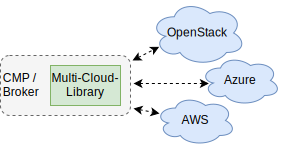
\includegraphics[width=0.48\textwidth]{images/multi-cloud-library.pdf}
	\def\svgwidth{0.75\textwidth}
	{\footnotesize \textsf{
			\includesvg{images/hyrise-r-deployment}}}
	\caption{Test-Deployment mit zwei Hyrise-R-Clustern, verteilt auf eine Public- und eine Private-Cloud. Orchestriert werden beide Services durch die selbstentwickelte Cloud-Management-Plattform aus der Private-Cloud heraus -- sie überwindet Provider- und Infrastrukturgrenzen.}	
	\label{fig:hyrise-r-deployment}
	%\end{wrapfigure}
\end{figure}

Der Dispatcher empfängt alle Anfragen an den Hyrise-R-Cluster. Jede Anfrage mit Schreibanteil leitet der Dispatcher an den Master-Knoten. Hier wird die Anfrage bearbeitet, in das Log geschrieben und anschließend mit allen Replicas synchronisiert. Enthält eine Anfrage nur Leseanteile, verteilt der Dispatcher sie an einen beliebigen Knoten.

% query performacne und synchronisations overhead.
Wir starten Hyrise-R immer als Cluster aus Dispatcher, Master und drei Replicas oder skalieren dynamisch je nach Leistungsanforderungen und SLO-Bedingungen.

1. Betrieb über Cloud-Grenzen hinweg
2. Betrieb auf heterogener Infrastruktur
3. Skalieren nach Leistungsanforderungen
4. Skalieren nach SLOs und Nutzeranforderungen
% Hier: Startzeit des Clusters als Metrik zur Bewertung des Brokerings. Stark abhängig von der Performance der Cloud-Infrastruktur und Netzwerverbindungen.
%Gemessen wird also nicht die Synchronisationszeit der Hyrise-R-Lösung, sondern die Skalierungsfähigkeiten der verwendeten Cloud-Lösungen und Orchestrierungstechniken.

HTTP-Schnittstelle empfängt Anfragen im JSON-Format: NoOp startet keine Datenbank-Operation, durchläuft aber alle Datenbankkomponenten von HTTP-Handling über Parser bis Executor.

Python-Code überarbeitet und parallelisiert.


Stattdessen wollen wir eine echte Anfrage Ausführen. Dazu nutzen wir die vorbereitete Beispieldatenbank und Anfrage aus einer früheren Arbeit.

Um sowohl OLTP- als auch OLAP-Fähigkeiten der In-Memory-Datenbank zu überprüfen, nutzen vorherige Arbeiten \cite{ssiclops:d42:experiments-measurements} den CH-benCHmark der TU München \cite{cole:2011:db-benchmark}. Dieser ist eine Mischung aus Transaktions- und Analysebenchmark, angelehnt an den hybriden Einsatz aktueller Datenbanksysteme in Unternehmen: Die gleichen Tabellen eines einzigen Datenbanksystems erfüllen alle Aufgaben des täglichen Geschäfts und liefern gleichzeitig umfassende Analysen. Trotzdem bleibt die Vergleichbarkeit des Benchmarks mit klassischen, getrennten Systemen.

Die Beispieldatenbank enthält eine Auftragshistorie mit knapp 300\,000 Datensätzen. Jede Zeile besteht aus sieben zufälligen Integer-, zwei String- und einem Float-Wert. So ergibt sich eine Rohgröße von 21,3\,MB. Die Beispielanfrage\footnote{\url{https://db.in.tum.de/research/projects/CHbenCHmark/}} liefert alle Bestellungen eines bestimmten Zeitraumes, sowie Summe, Gesamt- und Durchschnittswert aller enthaltenen Posten. Sie dient uns als \emph{Smoke-Test} -- liefert der Hyrise-R-Cluster eine valide Antwort im vorgegebenen Zeitrahmen, ist die generelle Funktionsfähigkeit gegeben und das Deployment erfolgreich abgeschlossen:

\begin{minted}{sql}
SELECT ol_number,
       SUM(ol_quantity) AS sum_qty,
       SUM(ol_amount)   AS sum_amount,
       AVG(ol_quantity) AS avg_qty,
       AVG(ol_amount)   AS avg_amount,
       COUNT(*)         AS count_order
FROM orderline 
WHERE ol_delivery_d > '2007-01-02 00:00:00.000000' 
GROUP BY ol_number
ORDER BY ol_number
\end{minted}


%Kosten: Rechenzeit und Bandbreite (außerhalb einer Cloud) also gegenläufiges Ziel zu Portabilität und Ausfallsicherheit, denn die geringsten Kosten fallen bei dem Betrieb in einer einzelnen Cloud eines Providers an.
%i) providers’ pricing models, (ii) application’s communication patterns and (iii) distribution of nodes over providers.
%https://www.google.de/url?sa=t&rct=j&q=&esrc=s&source=web&cd=1&ved=0ahUKEwju27vHs6DZAhUCWRQKHRv7BEcQFggrMAA&url=http%3A%2F%2Fwww.mikesmit.com%2Fwp-content%2Fpapercite-data%2Fpdf%2Fcloud2012.pdf&usg=AOvVaw3e6yhHYmhWBbIxtr7MqkuX

%verschiedene OpenStack-Versionen haben unterschiedliche Schnittstellen. Auch dies kann über die Middleware abgefangen werden. RefStack testet API, Rally testet performance und führt tempest-Tests aus.


Aufwand einer Multi-Cloud-Strategie

Umsetzung der Policys

Potential

Vorteile durch Multi-Cloud-Bibliotheken

Aufwand für ein Multi-Cloud-Testbed

Redundanz fehlt: Auch die CMP muss in einer vertrauenswürdigen Umgebung repliziert werden und synchronisieren. Dem Hyrise-R-Dispatcher fehlt diese Funktion ebenso.
	\chapter{Test und Diskussion}

\todo{Intro, Motivation, Überblick}

\section{Public-Cloud: AWS-Testbed}
\label{sec:aws-testbed}

Die Amazon-Web-Services-Integration ist eine besondere Herausforderung: Der komplette Auf- und Abbau der Testinfrastruktur benötigt mehrere Minuten. Zusätzlich kostet jede Ressourcennutzung Geld, unabhängig vom Zweck. Zwar stellt Amazon einmalig 100 Dollar Testbudget zur Verfügung; bei mehreren Hyrise-Instanzen sind diese jedoch innerhalb weniger Tage aufgebraucht. Durch die komplexe Struktur der Amazon-Dienste entsteht -- gerade während der Entwicklung des Cloud-Adapters -- ein hohes Kostenrisiko. Der Amazon-Container-Dienst ECS setzt immer eine gestartete Instanz der Elastic Compute Cloud (EC2) voraus. Diese verursacht auch Kosten, wenn kein Container ausgeführt wird. Damit ist das AWS-Verhalten nicht intuitiv und steht in Gegensatz zur \emph{On-Demand}--Philosophie.

Um Aufwand und Risiko zu senken, eignen sich teil-funktionale Platzhalter-Bibliotheken, sogenannte \emph{Mocks}. Sie implementieren die gleichen Schnittstellen wie herstellereigene Originale und beantworten Anfragen entsprechend -- jedoch ohne tatsächlich eine Netzwerkverbindung und entfernte Ressourcen zu nutzen. Für AWS existieren zwei interessante Projekte; \emph{Moto}\footnote{\url{http://docs.getmoto.org/en/latest/}} und \emph{LocalStack}\footnote{\url{https://localstack.cloud/}}. 

Moto ist eine Python-Bibliothek, die AWS-Aufrufe per Decorator oder Context-Manager direkt im Quellcode umleitet. Der angedachte Anwendungsfall ist die Kombination mit \emph{boto}, dem offiziellen AWS-Python-SDK\footnote{\url{https://aws.amazon.com/de/sdk-for-python/}}.

LocalStack ist  bibliotheks- und programmiersprachen-unabhängig. Es erstellt HTTP-Endpunkte für alle AWS-Dienste. Änderungen im Quellcode der eigentlichen Anwendung sind dafür nicht nötig. Daher ist auch eine Kombination mit Libcloud denkbar, um den Aufwand der AWS-Integration erheblich zu senken. Insgesamt erfordert die Arbeit mit AWS viel Aufmerksamkeit -- die wir lieber in die Konzeption des Brokers investieren. Im lokalen Test- und Entwicklungs-Set-up nutzen wir deshalb Docker als Amazon-ECS-Ersatz.

Für OpenStack sind keine derartig ausgereiften Mock-Projekte bekannt. Alle offiziellen Bibliotheken dienen eher zum Test der OpenStack-Komponenten selbst. Eine tatsächliche Ausführung von Gastanwendungen ist nicht vorgesehen. Um die Funktion mit OpenStack zu validieren, erstellen wir später unser eigenes Testbed im \autoref{sec:openstack-testbed}. Längerfristig wollen wir von Libcloud profitieren, da der Implementierungsaufwand nur einmalig anfällt. Anschließend existiert die Abstraktionsebene unabhängig von potenziellen Schnittstellenänderungen eines Cloud-Providers.

\section{Private-Cloud: OpenStack-Testbed}

Als Beispiel für eine Private-Cloud -- als Teil unseres Multi-Cloud-Setups -- soll OpenStack dienen. Es ist das populärste Open-Source-Projekt um eigene Infrastruktur als Service aufzubauen. Gesponsert wird es von Großunternehmen wie \emph{HPE}, \emph{IBM}, \emph{Canonical}, \emph{Red Hat} und anderen.

OpenStack setzt sich aus verschiedenen Teilprojekten zusammen, die jeweils einen Dienst entwickeln und bereitstellen. Ein Minimal-Setup besteht aus \emph{Nova} (Computing), \emph{Key\-stone} (Authentifizierung), \emph{Neutron} (Netzwerk) und \emph{Glance} (Images). Verbreitet sind außerdem \emph{Cinder} (Blockspeicher) und \emph{Horizon} (Dash\-board). Diese sollen auch in unserem Beispiel genutzt werden. Denkbar ist darüber hinaus die Integration eines Container-Dienstes. Der Zugriff auf die Infrastruktur erfolgt entweder über das Dashboard, Kommandozeilentools oder eine REST-API.

Grundsätzlich wäre auch der Aufbau einer OpenStack-Föderation wie in \emph{SSICLOPS} denkbar \cite{ssiclops:2015:d6.1-project-presentation}. Föderierte Cloud-Architekturen teilen sich zentrale Komponenten, in OpenStack mindestens den Authentifizierungsservice \emph{Keystone}. Je nach Föderationsvariante (\emph{Cells}, \emph{Regions}, \emph{Availability Zones} oder \emph{Host Aggregates}) sind auch Dienste wie Dashboard oder Speicher nur einmal vorhanden. Diese Architektur reduziert Fixkosten, erfordert allerdings spezielle Anpassungen innerhalb der Cloud. Auch gehen einige Vorteile wie Ausfallsicherheit und Unabhängigkeit der zentralen Dienste wieder verloren. Eine Kombination mit weiteren Cloud-Providern im Rahmen unseres Multi-Cloud-Setups ist denkbar, bleibt aufgrund der aufwendigen Einrichtung aber außen vor. Auch wäre der zusätzliche Erkenntnisgewinn vermutlich gering.\todo{SSICLOPS-OS-Architektur}

Selbst ein minimales OpenStack-Testsetup ist durch die diversen Dienste komplex. Denkbar wäre also auch die Nutzung von externen OpenStack-Angeboten. In diesem Projekt gibt es hierfür grundsätzlich drei mögliche Bereitstellungsmodelle: 

\begin{enumerate}
	\item Public Cloud
	\\\emph{Betrieb auf geteilter Cloud-Infrastruktur}
	
	\item Hosted Private Cloud
	\\\emph{Betrieb auf exklusiver Cloud-Infrastruktur}
	
	\item Lokale Testinstallation
	\\\emph{Betrieb auf eigener physischer oder virtueller Infrastruktur}
\end{enumerate}

\noindent Eine Liste öffentlicher OpenStack-Angebote findet sich auf der Projekthomepage\footnote{\url{https://www.openstack.org/marketplace/hosted-private-clouds/}}. Dort werden auch weitere Informationen wie Funktionsumfang und Zertifizierungen aufgeführt. 

Interessant ist zum Beispiel das Angebot der Deutschen Telekom \emph{Open Telekom Cloud\footnote{\url{https://cloud.telekom.de/en/infrastructure/open-telekom-cloud/}}}: eine Public Cloud auf OpenStack-Basis -- in Deutschland -- mit vollem Funktionsumfang und API-Zugriff. International bietet \emph{Rackspace} eine Hosted Private Cloud\footnote{\url{https://www.rackspace.com/openstack/}}. Beide eignen sich jedoch kaum, um kleine Experimente zu starten, sondern richten sich vor allem preislich an größere Organisationen und Unternehmen.

Kostenlos ist das Public-Cloud-Angebot \emph{TryStack}\footnote{\url{http://trystack.org/}}. Sponsoren wie \emph{Cisco}, \emph{NetApp}, \emph{Dell} und \emph{Red Hat} finanzieren das Projekt. Die Registrierung erfolgt über die Aufnahme in eine Facebook-Gruppe, anschließend soll hierüber auch der Zugang zur kostenlosen OpenStack-\emph{Liberty}-Instanz erfolgen. Während der gesamten Laufzeit dieser Arbeit war allerdings weder ein Login noch Kontakt zu den Organisatoren möglich.

Lokale OpenStack-Installationen sind aufwendig: Für jeden Dienst muss ein eigener physikalischer Rechner bereitstehen. Dementsprechend verweist die offizielle Dokumentation direkt auf die Vielzahl von OpenStack-Distributionen\footnote{\url{https://www.openstack.org/marketplace/distros/}}. Diese bieten fast immer einen vereinfachten Setup-Prozess und oft die Option statt physikalischen Rechnern virtuelle Maschinen oder Container zu nutzen. Wie auch bei den Hosted-Angeboten sind hier nicht alle Dienste verfügbar. In allen Paketen fehlt \emph{Zun}, der aktuelle Container-Service.

Speziell für lokale Test- und Entwicklungsumgebungen existiert \emph{DevStack}\footnote{\url{https://docs.openstack.org/devstack/latest/}}. Das offizielle OpenStack-Projekt installiert automatisiert die wichtigsten OpenStack-Dienste auf einer einzigen Maschine. Ausdrücklich unterstützt werden dabei auch VMs und \emph{LXC}-Container. Es soll daher als Erstes erprobt werden.

\section{DevStack virtualisiert inkl. Container-Support}

Während der Installation nimmt DevStack tief greifende Veränderungen am Hostsystem vor. Es müsste also auf einem separaten Server installiert werden. Dieser Abschnitt beschreibt den Versuch einer virtualisierten, reproduzierbaren DevStack-Testinstallation. Außerdem soll \emph{Zun} integriert werden. 

Ziel ist DevStack in einem Container auszuführen, genauso wie die darin gestarteten Compute-Nodes ebenso in einem -- nun verschachtelten -- Container bereitzustellen. Die Gründe hierfür sind zusammengefasst:

\begin{enumerate}
	\item Keine oder minimale Änderungen am Hostsystem
	\item Reproduzierbarer Testaufbau
	\item Schneller und rückstandsloser Reset
	\item Zustände (\emph{Snapshots}) speicherbar
	\item Schnelle Ausführung von Gastapplikationen
\end{enumerate}

\noindent Auch eine virtuelle Maschine löst die oben genannten Probleme. Theoretisch. Problematisch wird die Ausführungsgeschwindigkeit von Gastanwendungen in einem mit \emph{VirtualBox} virtualisierten OpenStack. Eine Lösung ist \emph{verschachteltes KVM}, das bereits in einer Arbeit erprobt wurde [1]. Die Autoren empfehlen ihren Vorschlag bei bestehenden Erfahrungen mit \emph{libvirt}. Der damalige Versuchsaufbau stellt sich allerdings als instabil und nicht mehr reproduzierbar heraus.

\begin{figure}[ht]
	\centering
	\begin{subfigure}[b]{0.29\textwidth}
		\def\svgwidth{\linewidth}
		{\tiny \textsf{
			\includesvg{images/devstack-bare-metal}}}
		\caption{Bare-Metal-Installation}
		\label{fig:sub:devstack-bare-metal}
	\end{subfigure}\hfill%
	\begin{subfigure}[b]{0.31\textwidth}
		\def\svgwidth{\linewidth}
		{\tiny \textsf{
			\includesvg{images/devstack-vm}}}
		\caption{All-in-One-VM}
		\label{fig:sub:devstack-vm}
	\end{subfigure}\hfill%
	\begin{subfigure}[b]{0.31\textwidth}
		\def\svgwidth{\linewidth}
		{\tiny \textsf{
			\includesvg{images/devstack-docker}}}
		\caption{DevStack in Docker}
		\label{fig:sub:devstack-docker}
	\end{subfigure}
	
	\caption{Verschiedene Installationsvarianten für eine OpenStack-Testinstallation mit DevStack auf einem einzelnen Host -- inklusive Unterstützung für Docker-Compute-Container und klassische VMs. Eine direkte Installation verändert unwiderruflich das gesamte Host-System \emph{(a)}. Eine VM benötigt mehr Ressourcen und kann die Geschwindigkeit der Gastanwendungen negativ beeinflussen \emph{(b)}. Die Installation in einem Container schafft Abstraktion und Reproduzierbarkeit ohne Geschwindigkeitskompromisse. Die Gastcontainer nutzen weiterhin den Kernel des Host-OS \emph{(c)}.}
	\label{fig:devstack}
\end{figure}

\emph{LXD}-Container könnten sich ebenfalls eignen. Im Gegensatz zu Docker führen sie mehrere Prozesse aus, erinnern also mehr an eine klassische virtuelle Maschine (ohne deren Overhead). Laut Entwickler \emph{Canonical} fokussiert sich \emph{LXD} speziell auf IaaS-Aufgaben\footnote{\url{https://www.ubuntu.com/containers/lxd}}. Ein LXD-DevStack-Setup birgt allerdings die gleichen Hürden\footnote{\url{https://docs.openstack.org/devstack/latest/guides/lxc.html}} wie ein Docker-Setup \cite{graber:2016:openstack-lxd}. Nennenswert ist noch das OpenStack-Projekt \emph{Kolla}, das jeden OpenStack-Dienst in einem eigenen Docker-Container installiert\footnote{\url{https://cloudbase.it/openstack-kolla-hyper-v/}}.

Um Container innerhalb von OpenStack auszuführen, gibt es mehrere, teils konkurrierende Projekte. Alle lassen sich über Plugins in DevStack einbinden. Zu den Wichtigsten gehören \cite{singh:2017:containers-openstack}:

\begin{description}
	
	\item[Zun\footnotemark]\footnotetext{\url{https://wiki.openstack.org/wiki/Zun}} Eigenständige OpenStack-API zum Starten und Verwalten von diversen Containertypen, inklusive \emph{Docker}.
	
	\item[Nova Docker\footnotemark]\footnotetext{\url{https://wiki.openstack.org/wiki/Docker}} Im Gegensatz zu \emph{Zun} erfolgt die Docker-Containerverwaltung über die bekannte Nova-API. Das Projekt wurde eingestellt.
	
	\item[Nova LXD\footnotemark]\footnotetext{\url{https://linuxcontainers.org/lxd/getting-started-openstack/}} Parallel zu \emph{Nova Docker} erfolgt der Zugriff über die Nova-API. Das Projekt wird von \emph{Canonical} aktiv vorangetrieben. Weiterer Teil ist die Automatisierung via \emph{Juju}.
	
	\item[Magnum\footnotemark]\footnotetext{\url{https://wiki.openstack.org/wiki/Magnum}} Eine Self-Service-Lösung zur Orchestrierung auf Basis von \emph{Heat}. Stellt automatisiert Container Orchestration Engines (COEs) wie \emph{Docker Swarm} und \emph{Kubernetes} bereit.
	
\end{description}

DevStack in Docker wurde bereits vor einiger Zeit umgesetzt\footnote{\url{https://github.com/ewindisch/dockenstack}}. Da das Projekt nicht mehr gepflegt wird und auf das ebenfalls beendete \emph{Nova Docker} aufsetzt, erfolgt die Neuimplementierung mit folgenden Änderungen:

\begin{itemize}
	
	\item Ubuntu-LTS-Basis-Image 14.04 $\Rightarrow$ 17.10
	\item Mehrprozessunterstützung per \emph{systemd}\footnote{\url{https://docs.openstack.org/devstack/latest/systemd.html}}
	\item OpenStack-Version Kilo $\Rightarrow$ Pike
	\item libvirt/QEMU-Instanzen
	\item Nova Docker $\Rightarrow$ Zun
	\item Container-angepasste DevStack-Konfiguration
	\item Vollständige Netzwerkkonfiguration
	
\end{itemize}

Größte Hürde ist die Limitierung auf einen Prozess innerhalb eines Standard-Docker-Containers. Neuere DevStack-Versionen setzen auf \emph{systemd}. Daher muss dies über die Umgebungsvariable \emph{ENV container docker} bekannt gemacht werden. Anschließend lässt sich \emph{systemd} über zwei weitere Workarounds starten\footnote{\url{https://github.com/moby/moby/issues/27202}}\footnote{\url{https://github.com/moby/moby/issues/9212}}.

\emph{Docker Build} bereitet das Image mit allen externen DevStack-Abhängigkeiten vor. Notwendige Dienste wie \emph{RabbitMQ} und \emph{MySQL} werden bereits im Voraus installiert. Das Container-Image führt beim Start nur noch die allerletzten Schritte des Setups aus. Ganz vorweg nehmen lässt sich das Setup nicht, weil während des Builds keine erweiterten Rechte vorliegen.

Nach erfolgreichem Start reicht das Kommando \emph{make run}, um per Zun einen \emph{Cirros}-Basis-Container\footnote{\url{https://docs.docker.com/samples/library/cirros/}} zu starten. Der Stand der gesamten OpenStack-Installation lässt sich per \emph{docker commit} oder experimentell per \emph{Docker-Snapshots}\footnote{\url{https://criu.org/Docker}} sichern.

Anpassbar sind im Skript OpenStack-Services und -Versionen, da DevStack direkt aus den Quellen installiert wird. So ändern sich allerdings selbst die Abhängigkeiten der als stabil gekennzeichneten Versionen. Das Prinzip Infrastruktur als Code geht hier nicht immer auf -- DevStack ist nicht zuverlässig reproduzierbar. \autoref{fig:devstack} vergleicht die Installationsvarianten.

Als \emph{Proof-of-Concept} ist die Integration von Docker, DevStack und Zun bisher einmalig. Der Code ist daher auf GitHub\footnote{\url{https://github.com/janmattfeld/DockStack}} veröffentlicht und zeigt einige \emph{Best Practices} und \emph{Lessons Learned} in Bezug auf die genannten Projekte.

Zusätzlich greifen wir auf eine lokale \emph{Mirantis}-OpenStack-Installation aus dem \emph{SSICLOPS}-Projekt zurück. Die Infrastruktur ist virtuell und wird durch \emph{Fuel}\footnote{\url{https://www.mirantis.com/software/openstack/}} zuverlässiger wieder aufgebaut. Die Zun-Container-Dienste sind aufgrund der älteren OpenStack-Version nicht enthalten; dafür aber alle anderen Kernfunktionen und APIs.


\section{Testanwendung: Hyrise-R}
\label{sec:hyrise-r}

Hyrise\footnote{\url{https://hpi.de/plattner/projects/hyrise.html}} ist eine In-Memory-Forschungsdatenbank der Fachgruppe \emph{Enterprise Platform and Integration Concepts (EPIC)} am Hasso-Plattner-Institut \cite{grund:2010:hyrise}. Die Datenbank teilt sich einige Eigenschaften mit \emph{SAP HANA}\footnote{\url{https://www.sap.com/products/hana.html}}: Ein \emph{Delta Store}, spaltenorientierte Speicherung, Wörterbuchkodierung und weitere Komprimierungstechniken sowie den \emph{Insert-Only}-Ansatz und Partitionierung. Herausragend ist die OLAP-Performance, enthalten sind aber auch Optimierungen für OLTP-Aufgaben.

Hyrise-R ist eine Erweiterung des Basisprojektes um Replikation \cite{schwalb:2015:hyrise-r}. Es folgt dabei dem \emph{Scale-Out}-Ansatz: Alle schreibenden Operationen werden auf einem einzigen \emph{Master-Node} durchgeführt. Dessen Datensatz wird in weniger als einer Sekunde (\emph{lazy}) mit beliebig vielen \emph{Replica-Nodes} abgeglichen. Diese Spiegelungen bearbeiten alle reinen Leseanfragen und machen den Verbund so skalierbar, siehe \autoref{fig:hyrise-r}. Nach dem \emph{CAP-Theorem} sind Verfügbarkeit und Partitionstoleranz hier also wichtiger als Konsistenz. 

\begin{figure}[ht]
	\centering
	\def\svgwidth{0.9\textwidth}
	\textsf{
	\includesvg{images/hyrise-r}}
	\caption{Verteilte \emph{Hyrise-R}-Architektur mit getrennter Verarbeitung von Lese- und Schreibanfragen. Der Master-Knoten dient als \emph{Single Source of Truth}. Zur Leistungssteigerung übernehmen Spiegelserver die Beantwortung der meisten Leseanfragen. Kleinere Inkonsistenzen werden dabei in Kauf genommen. Nicht im Bild ist der Dispatcher zur Anfrageverteilung. Aus \cite{ssiclops:d42:experiments-measurements}.}	
	\label{fig:hyrise-r}
\end{figure}

Durch die verteilte Architektur ist Hyrise-R ein potenzieller Kandidat als Testanwendung innerhalb der Multi-Cloud-Umgebung. Einige \emph{SSICLOPS}-Teilprojekte untersuchten bereits Zuverlässigkeit, Performance, Datensicherheit und Vertraulichkeit in einer privaten OpenStack-Föderation \cite{ssiclops:d23:security-extensions, ssiclops:d42:experiments-measurements, bastian:2017:openstack-policies}.

Im Rahmen dieser Arbeiten sind einige Infrastrukturteile als Code veröffentlicht: So existiert zum Beispiel eine Docker-Teststellung mit grafischem Cluster-Manager, um die Performance bei verschiedenen Replikationsstufen zu prüfen. Diese Infrastruktur wurde in mehreren Studienarbeiten weiter angepasst, um Hyrise-R-KVM-Images in OpenStack bereitzustellen \cite{eschrig:2016:ssiclops-masterproject, maschler:2017:ssiclops-masterproject}.

Um als Testanwendung über mehrere Cloud-Ebenen zu dienen, sollte Hyrise-R auf den verbreiteten Hypervisoren, IaaS- und CaaS-Providern ausführbar sein. Aufgrund der Softwarestruktur, als eigenentwickelte \emph{Low-Level-C++-Anwendung}, eignet Hyrise-R sich nicht direkt\footnote{\url{https://cloud.google.com/appengine/docs/flexible/custom-runtimes/}} als Testanwendung für PaaS-Angebote. Hierfür nutzen wir andere Standardsoftware, die auf den üblichen PaaS-Sprachen wie Java, Python oder Node.js aufbaut.

Hyrise-R ist von Anfang an für die Skalierung über externe Broker konzeptioniert. Die bisherigen Arbeiten haben \emph{Standalone-Cluster-Manager} umgesetzt, erst für Docker und später für OpenStack\footnote{\url{https://github.com/DukeHarris/hyrise_rcm}}\footnote{\url{https://github.com/SSICLOPS/openstack-testbed-vm}}. Die nötigen Clusterinformationen werden Hyrise-Instanzen direkt beim Start als Parameter übergeben. Variablen zur Laufzeitumgebung müssen während des Deployments vom Broker ausgefüllt werden: Konkret benötigt Hyrise einen TCP-Port und eine eindeutige Knoten-ID. Über ihre ID registrieren sich Knoten am Dispatcher. Hierzu benötigen sie dessen IP-Adresse und Port -- der Dispatcher muss also immer als Erstes in einem Cluster bereitstehen. Erst dann können Start und Registrierung des Masters erfolgen. Plattformunabhängig ergeben sich folgende Startskripte für einen Hyrise-R-Cluster:

\newpage
\begin{description}
	
\item[{[1]} Dispatcher] einmal pro Cluster, zentrale Lastverteilung für alle Anfragen
	
\begin{minted}{jinja}
./dispatcher {{dispatcher.port}} settings.json
\end{minted}
	
\item[{[1]} Master] einmal pro Cluster als \emph{Single-Source-of-Truth}, bearbeitet alle Schreibanfragen, gekennzeichnet durch \emph{nodeId=0}
	
\begin{minted}{jinja}
./hyrise \
  --dispatcherurl={{dispatcher.ip}} \
  --dispatcherport={{dispatcher.port}} \
  --nodeId=0 \
  --port={{master.port}}
\end{minted}

\item[{[0-n]} Replica] optional, beliebig viele Instanzen pro Cluster zur Entlastung des Master-Knotens bei Leseanfragen

\begin{minted}{jinja}
./hyrise \
  --dispatcherurl={{dispatcher.ip}} \
  --dispatcherport={{dispatcher.port}} \
  --nodeId={{replica.id}} \
  --port={{replica.port}}
\end{minted}
	
\end{description}

In vorherigen Projekten entwickelte Images für virtuelle Maschinen laufen auf der verbreiteten Hypervisorkombination aus QEMU und KVM. Die Erstkonfiguration erfolgte bisher über direkte SSH-Kommandos an die gestartete virtuelle Maschine. Dies erforderte die Konfiguration von SSH in den VMs und die Verwaltung von Schlüsseln in der CMP. Zusätzlich entstand eine Wartezeit zwischen VM-Startkommando und Erstkonfiguration, die vorherige Projekte durch Polling noch ausdehnten. Eine elegantere Lösung ist \emph{cloud-init}: Die CMP füllt eine Konfigurationsvorlage und schickt es direkt im Startkommando an den Infrastruktur-Provider. Dieser führt das Skript ohne weitere Wartezeit aus.

Auch Docker-Images existieren bereits unverändert seit 2015\footnote{\url{https://github.com/hyrise/hyrise-v1/tree/feature/docker}}. In der Zwischenzeit wurden Docker, diverse Abhängigkeiten und Hyrise selbst allerdings weiterentwickelt. Innerhalb eines Clusters sollten alle Knoten dieselbe Hyrise-Version ausführen. Daher aktualisieren wir Dispatcher und Hyrise auf Basis des aktuellsten Hyrise-NVM-Branches\footnote{\url{https://github.com/janmattfeld/dispatcher/tree/docker}}\footnote{\url{https://github.com/janmattfeld/hyrise_nvm/tree/feature/docker}}.

Die Aktualisierung enthält das aktuelle Docker-Basis-Image Ubuntu\,16.04. Wir integrieren außerdem korrekte Metadaten und Dokumentation zur Imageerstellung und Ausführung. Einige eingebundene Git-Submodule wurden in der Zwischenzeit verschoben oder existieren nicht mehr -- die verwendete CSV-Bibliothek muss zum Beispiel ausgetauscht werden. Dies erfordert kleinere Änderungen am Quellcode. Genauso wie neue \emph{Non-Uniform-Memory-Access-Funktionen (NUMA)}: Die Funktion \emph{membind} erfordert erweitere Rechte. In einem Standard-Docker-Container sind diese aber nicht vorhanden. Der neue Startparameter \mbox{\emph{-\,-disable\_membind}} deaktiviert die speziellen NUMA-Funktionen. Unsere Images laufen daher auch in Container-Laufzeitumgebungen der Public-Cloud-Provider.

Das Image ist zum Produktivbetrieb gedacht: Docker Build entfernt nach dem Image-Erstellungsprozess alle Abhängigkeiten, die zum Betrieb nicht notwendig sind. So reduziert sich die Image-Größe von über 500 auf weniger als 300\,MB -- entsprechend verkürzt sich die Startzeit. Enthalten ist außerdem eine Beispieldatenbank, die wir später als Benchmark und initialen Funktionstest nutzen werden. Gemessen wird also nicht die Synchronisationszeit der Hyrise-R-Lösung, sondern die Skalierungsfähigkeiten der verwendeten Cloud-Lösungen und Orchestrierungstechniken. Wir setzen außerdem pragmatische Startparameter für Hyrise-R auf Docker: \emph{-\,-corecount=2} \emph{-\,-disable\_membind}. Die neuen Images sind zur leichteren Integration auf Docker Hub veröffentlicht\footnote{\url{https://hub.docker.com/r/hyrise/dispatcher/}}\footnote{\url{https://hub.docker.com/r/janmattfeld/hyrise_r/}}. Um auch zukünftige Weiterentwicklungen von Hyrise nutzen zu können, automatisiert ein neues Makefile Docker-Build-Voränge und den Realease auf Docker Hub.

\begin{figure}[ht]
	\centering
	\begin{subfigure}[b]{0.45\textwidth}
		\def\svgwidth{\linewidth}
		{\scriptsize \textsf{
				\includesvg{images/hyrise-r-runtime-vm}}}
		\caption{Virtuelle Maschine}
		\label{fig:sub:hyrise-r-runtime-vm}
	\end{subfigure}\hfill%
	\begin{subfigure}[b]{0.45\textwidth}
		\def\svgwidth{\linewidth}
		{\scriptsize \textsf{
				\includesvg{images/hyrise-r-runtime-docker}}}
		\caption{Container}
		\label{fig:sub:hyrise-r-runtime-docker}
	\end{subfigure}	
	\caption{Aktualisierte Ausführungsumgebungen für Hyrise-R-Master/Replica auf IaaS- und CaaS-Plattformen. Die Anmerkungen auf der linken Seite beschreiben verwendete Technologien und Schnittstellen.}
	\label{fig:devstack}
\end{figure}

Aus der bisher losen Sammlung von Quellcode, Shell-Skripten und Makefiles in mehreren GitHub-Repositorys haben wir eine nachhaltige Pipeline zur automatisierten Image-Erstellung für verschiedene Infrastrukturen entwickelt\footnote{\url{https://github.com/janmattfeld/hyrise_nvm/commit/cfe3aa8}}. Ausführungsumgebung, Programm, Testdaten und Konfiguration werden flexibel integriert -- Hyrise-R eignet sich nun als Testanwendung für den Multi-Cloud-Broker.

Als Weiterentwicklung zu den bisherigen Hyrise-R-Arbeiten soll der Broker nicht nur nach Leistungsanforderungen skalieren, sondern auch SLAs und Geostandorte beachten sowie diverse Infrastrukturanbieter nutzen.


\section{Praxis: Multi-Cloud-Brokering}
\label{sec:brokering-test}

In den vorherigen Abschnitten haben wir die Funktionsweise des Brokers erläutert, den modularen Vorschlag als Python-Service implementiert, sowie Hyrise-R zum Cloud-Betrieb vorbereitet. Auf dem virtualisierten OpenStack-Testbed soll nun die Funktionsweise des Gesamtsystems geprüft werden: Zwei Hyrise-R-Cluster laufen über zwei Clouds verteilt und werden dynamisch skaliert, siehe \autoref{fig:hyrise-r-deployment}.

\begin{figure}[ht]
	\centering
	\def\svgwidth{0.85\textwidth}
	{\scriptsize \textsf{
			\includesvg{images/hyrise-r-deployment}}}
	\caption{Testarchitektur mit zwei Hyrise-R-Clustern, verteilt auf eine Public- und eine Private-Cloud. Cluster \emph{B} nutzt AWS, um unkritische Daten kostengünstig auszulagern. Orchestriert werden beide Services durch die selbst entwickelte Cloud-Management-Plattform aus der Private-Cloud heraus -- die CMP harmonisiert Provider- und Infrastrukturgefälle.}	
	\label{fig:hyrise-r-deployment}
\end{figure}

Wir starten Hyrise-R immer als Cluster aus Dispatcher, Master und einer per SLO-Vorlage bestimmten Anzahl an Replika. Anschließend skalieren wir den Cluster dynamisch nach Leistungsanforderungen und SLO-Bedingungen. Das erneute Starten anhand von veränderter Umgebung ist eingeschränkt: Hyrise-R unterstützt keine Echtzeitmigration. Einzig die Replika lassen sich ohne Probleme an- und abmelden -- für Tests des Cloud-Burstings, also dem Abfangen erhöhter Last durch weitere Instanzen, ist das kein Problem. Entweder der Broker sucht eine passende Infrastruktur und startet einen neuen Hyrise-R-Replika-Knoten, oder er fährt einen Knoten herunter und meldet ihn ab. Die Tests sind rein qualitativ und decken folgende Fälle ab:

\begin{enumerate}
	\item Betrieb über Cloud-Grenzen hinweg
	\item Betrieb auf heterogener Infrastruktur
	\item Skalieren nach Leistungsanforderungen
	\item Skalieren nach weiteren SLOs und Nutzeranforderungen
\end{enumerate}

In einem funktionsfähigen Hyrise-R-Cluster empfängt der Dispatcher alle Anfragen. Jede Anfrage mit Schreibanteil leitet er an den Master-Knoten. Hier wird die Anfrage bearbeitet, in das Log geschrieben und anschließend mit allen Replika synchronisiert. Enthält eine Anfrage nur Leseanteile, verteilt der Dispatcher sie an einen beliebigen Knoten. Frühere Arbeiten bewerteten an dieser Stelle die Anfrageperformance und den Synchronisationsoverhead. Beide Metriken sind jedoch stark abhängig von der Performance der Cloud-Infrastruktur und Netzwerkverbindungen.

Als Metrik zur Bewertung des Brokerings gilt -- neben Einhaltung der SLOs -- die volle Funktionsfähigkeit des Clusters. Eine Beispieldatenbank ist bereits in den Images enthalten. Alle Anfragen haben ausschließlich lesende Anteile, die Tabelle wird nicht durch Schreibanfragen verändert und muss deshalb nicht synchronisiert werden. Gemessen wird also nicht die Synchronisationszeit der Hyrise-R-Lösung, sondern die Skalierungsfähigkeiten der verwendeten Cloud-Lösungen und Orchestrierungstechniken.

Die Hyrise-HTTP-Schnittstelle empfängt Anfragen im JSON-Format. Die minimale Anfrage \emph{NoOp} startet keine Datenbankoperation, durchläuft aber alle Datenbankkomponenten von HTTP-Handling über Parser bis Ausführungseinheit. Als erster Funktionstest würde diese Anfrage genügen. Wir möchten allerdings den gesamten Cluster testen, und nutzen daher eine echte, hinreichend komplexe Anfrage. Deren Bearbeitung benötigt genug Zeit, damit der Dispatcher sie auf alle Knoten aufteilen kann. Den vorhandenen Python-Code überarbeiten und parallelisieren wir. Die Anzahl der Knoten lässt eine bestimmte Performance erwarten -- für einen gültigen Test muss die Anzahl der Anfragen mindestens der Anzahl Knoten entsprechen:

\begin{minted}{python3}
queries = [(host, port, query)] * num_nodes
start_time = time.time()
with multiprocessing.dummy.Pool(num_threads) as pool:
	pool.starmap(query_hyrise, queries)
queries_second = num_nodes / (time.time() - start_time)
\end{minted}

Um sowohl OLTP- als auch OLAP-Fähigkeiten der In-Memory-Datenbank zu überprüfen, nutzen vorherige Arbeiten \cite{ssiclops:d42:experiments-measurements} den CH-benCHmark der TU München \cite{cole:2011:db-benchmark}. Dieser ist eine Mischung aus Transaktions- und Analysebenchmark, angelehnt an den hybriden Einsatz aktueller Datenbanksysteme in Unternehmen: Die gleichen Tabellen eines einzigen Datenbanksystems erfüllen alle Aufgaben des täglichen Geschäfts und liefern gleichzeitig umfassende Analysen. Trotzdem bleibt die Vergleichbarkeit des Benchmarks mit klassischen, getrennten Systemen.

Die Beispieldatenbank enthält eine Auftragshistorie mit knapp 300\,000 Datensätzen. Jede Zeile besteht aus sieben zufälligen Integer-, zwei String- und einem Float-Wert. So ergibt sich eine Rohgröße von 21,3\,MB. Die folgende Beispielanfrage\footnote{\url{https://db.in.tum.de/research/projects/CHbenCHmark/}} zeigt alle Bestellungen eines bestimmten Zeitraumes, sowie Summe, Gesamt- und Durchschnittswert aller enthaltenen Posten. Sie dient uns als \emph{Smoke-Test} -- liefert der Hyrise-R-Cluster eine valide Antwort im vorgegebenen Zeitrahmen, ist die generelle Funktionsfähigkeit gegeben, und das Deployment erfolgreich abgeschlossen:

\begin{minted}{sql}
SELECT ol_number,
       SUM(ol_quantity) AS sum_qty,
       SUM(ol_amount)   AS sum_amount,
       AVG(ol_quantity) AS avg_qty,
       AVG(ol_amount)   AS avg_amount,
       COUNT(*)         AS count_order
FROM orderline 
WHERE ol_delivery_d > '2007-01-02 00:00:00.000000' 
GROUP BY ol_number
ORDER BY ol_number
\end{minted}

%To-do: Konkreter Test, SLOs: Verlinken aus vorherigem Abschnitt. Forschungshypothese: Steigerung von  Datensicherheit, Vertraulichkeit und Portabilität.

\noindent
Das folgende Minimalbeispiel ist der Smoke-Test unseres Prototyps:
\begin{minted}{python}
init_clouds(filter=['ecs', 'openstack'])
deploy_app('hyrise')
validate_throughput('hyrise')
teardown(filter='all')
\end{minted}

\noindent
Um die, in \autoref{cha:implementierung} vorgestellten, Strategien zu Platzierung und anschließender Skalierung zu überprüfen, definieren wir zwei umfangreichere Testfälle, siehe \autoref{tab:testcases}. Der gerade diskutierte Hyrise-R-Benchmark dient dabei zur Bestimmung der Durchsatz-Qualitätsvereinbarung. Gleichzeitig nutzen wir alle definierten Komponenten des Brokers sowie unsere kombinierten Anwendungs- und SLA-Vorlagen.  Welche Stärken und weiteren Herausforderungen der Test zeigt, diskutiert der nächste Abschnitt.

\begin{table}[h!]
\centering%
\ra{1.3}%
\caption{Testfälle der beiden zentralen Broker-Funktionen.}%
\begin{tabularx}{\textwidth}{LLLLL}%
\toprule%
%
Test Case & Clouds & Policies & SLAs & Optimization\\%
%
\midrule%
%
Placement & OpenStack, AWS ECS & Geo, Replication & -- & Pricing\\%
Scaling   & OpenStack, AWS ECS & Geo, Replication, Workload & Throughput & Pricing\\%
\bottomrule%
\end{tabularx}
\label{tab:testcases}
\end{table}


\section{Stärken und Herausforderungen}

%verschiedene OpenStack-Versionen haben unterschiedliche Schnittstellen. Auch dies kann über die Middleware abgefangen werden. RefStack testet API, Rally testet performance und führt tempest-Tests aus.


Aufwand einer Multi-Cloud-Strategie

Umsetzung der Policys
- Apps gemeinsam betrachten und optimieren
- Services gemeinsam betrachten und optimieren

Potenzial

Vorteile durch Multi-Cloud-Bibliotheken

Aufwand für ein Multi-Cloud-Testbed

Redundanz fehlt: Auch die CMP muss in einer vertrauenswürdigen Umgebung repliziert werden und synchronisieren. Dem Hyrise-R-Dispatcher fehlt diese Funktion ebenso.

% See IETF Inter Cloud Framework Requirements and Diagram S.26
%Cloud Services Layers (Logical) (Intercloud Communication)
	%In der Schlussbetrachtung gibt es einen Rückblick, in dem Motivation und Thesen aus der Einleitung wieder aufgegriffen und abgerundet werden. Antworten auf in der Problemstellung aufgeworfene Fragen werden kurz und prägnant zusammengefasst. Ebenso sollte ein Ausblick auf offen gebliebene Fragen sowie auf interessante Fragestellungen, die sich aus der Arbeit ergeben, gegeben werden. Ein persönlich begründetes Fazit aus eigener Perspektive ist an dieser Stelle ebenfalls sinnvoll.
%

\chapter{Zusammenfassung und Ausblick}

\begin{description}
	
	\item[Notfallplan] Bei Ausfall der gesamten Ausführungsplattform kann eine Migration zu einem anderen Anbieter erfolgen.
	
	\item[Abfangen von Lastspitzen] Zusätzliche Service-Instanzen auf externen Ressourcen bearbeiten bei Bedarf weitere Anfragen.
	
	\item[Lebenszyklus-Verwaltung] Typischerweise durchläuft eine neue Service-Version die Phasen Entwicklung, Test, Qualitätssicherung und Produktion. Hierfür existieren oft unterschiedliche Ausführungsumgebungen.
	
\end{description}

%Rightscale Video: https://www.rightscale.com/solutions/problems-we-solve/self-service-it

Einheitliche Standards zu Services, SLAs und Kommunikation.

Policys innerhalb von Instanzen 
%(allow SSH, check for security vulnerabilities)

Policys auf Datenebene

Ausbau zu einer produktiven CMP
Identity
Discovery
Monitoring
Dashboard
CAMP-Pläne zum Austausch mit weiteren Cloud-Management-Plattformen.

Trend: Serverless

Migrationshürden von Apps auf die CMP: OS Version, SSL-Zertifikate, statische und virtuelle IPs, Lizenzen, Load Balancing, Clustering, Bandbreite, Mandantenfähigkeit.

Failover-Handling nicht definiert. Im Moment: Bereitstellung eines Services mit der gleichen Adresse bei Ausfall. Weitere Arbeit auf Anwendungsebene (Hyrise-R) nötig. Oder Ausgliederung der Service-Discovery an ein externes Tool.

Überwachung der SLAs und Durchsetzen von Schadensersatz.
	
	% Bibliographie
	\ifisbook\cleardoubleemptypage\fi
	\phantomsection\addcontentsline{toc}{chapter}{\refname}
	\printbibliography[category=cited]

	% Eigenständigkeitserklärung
	\ifisbook\pagestyle{plain}\cleardoubleemptypage% => Laut Aussage des Studienreferats braucht es - auch wenn die Arbeit in englischer Sprache verfasst ist - KEINE separate Version der Eigenständigkeitserklärung auf Englisch. Sowohl für Arbeiten in deutscher Sprache als auch für Arbeiten in englischer Sprache genügt EINE EINZIGE Eigenständigkeitserklärung auf DEUTSCH.
\begin{otherlanguage}{ngerman}

\begin{center}\textsf{\textbf{Eidesstattliche Erklärung}}\end{center}
Hiermit versichere ich, dass meine {\hpitype} \enquote{\hpititle} (\enquote{\hpititleother}) selbständig verfasst wurde und dass keine anderen Quellen und Hilfsmittel als die angegebenen benutzt wurden. Diese Aussage trifft auch für alle Implementierungen und Dokumentationen im Rahmen dieses Projektes zu.\\

\noindent
Potsdam, den \hpidate,
\vspace{2cm}

\begin{center}
\begin{tabular}{C{6cm}}
\hline
{\small({\hpiauthor})}
\end{tabular}
\end{center}

\end{otherlanguage}


\fi

\end{document}